\documentclass[11pt,a4paper,twoside]{article}
\usepackage{lmodern}
\usepackage{amssymb,amsmath}
\usepackage{ifxetex,ifluatex}
\usepackage{fixltx2e} % provides \textsubscript
\ifnum 0\ifxetex 1\fi\ifluatex 1\fi=0 % if pdftex
  \usepackage[T1]{fontenc}
  \usepackage[utf8]{inputenc}
\else % if luatex or xelatex
  \ifxetex
    \usepackage{mathspec}
  \else
    \usepackage{fontspec}
  \fi
  \defaultfontfeatures{Ligatures=TeX,Scale=MatchLowercase}
\fi
% use upquote if available, for straight quotes in verbatim environments
\IfFileExists{upquote.sty}{\usepackage{upquote}}{}
% use microtype if available
\IfFileExists{microtype.sty}{%
\usepackage{microtype}
\UseMicrotypeSet[protrusion]{basicmath} % disable protrusion for tt fonts
}{}
\usepackage[left=2.5cm,right=3.5cm,top=83.75pt,textheight=24.35cm,textwidth=15cm,a4paper,headheight=13.6pt,twoside=true]{geometry}
\usepackage{hyperref}
\hypersetup{unicode=true,
            pdfborder={0 0 0},
            breaklinks=true}
\urlstyle{same}  % don't use monospace font for urls
\usepackage{biblatex}

\addbibresource{bibliography.bib}
\addbibresource{packages.bib}
\usepackage{longtable,booktabs}
\usepackage{graphicx,grffile}
\makeatletter
\def\maxwidth{\ifdim\Gin@nat@width>\linewidth\linewidth\else\Gin@nat@width\fi}
\def\maxheight{\ifdim\Gin@nat@height>\textheight\textheight\else\Gin@nat@height\fi}
\makeatother
% Scale images if necessary, so that they will not overflow the page
% margins by default, and it is still possible to overwrite the defaults
% using explicit options in \includegraphics[width, height, ...]{}
\setkeys{Gin}{width=\maxwidth,height=\maxheight,keepaspectratio}
\IfFileExists{parskip.sty}{%
\usepackage{parskip}
}{% else
\setlength{\parindent}{0pt}
\setlength{\parskip}{6pt plus 2pt minus 1pt}
}
\setlength{\emergencystretch}{3em}  % prevent overfull lines
\providecommand{\tightlist}{%
  \setlength{\itemsep}{0pt}\setlength{\parskip}{0pt}}
\setcounter{secnumdepth}{5}

%%% Use protect on footnotes to avoid problems with footnotes in titles
\let\rmarkdownfootnote\footnote%
\def\footnote{\protect\rmarkdownfootnote}

%%% Change title format to be more compact
\usepackage{titling}

% Create subtitle command for use in maketitle
\newcommand{\subtitle}[1]{
  \posttitle{
    \begin{center}\large#1\end{center}
    }
}

\setlength{\droptitle}{-2em}

  \title{}
    \pretitle{\vspace{\droptitle}}
  \posttitle{}
    \author{}
    \preauthor{}\postauthor{}
    \date{}
    \predate{}\postdate{}
  
\usepackage{booktabs}
\usepackage[ngerman,english]{babel} % deutsche Trennregeln, "Inhaltsverzeichnis" etc.
%\usepackage{mathptmx} % Times-Roman-Schrift (auch für mathematische Formeln)

\usepackage[labelfont=bf]{caption}
\usepackage[strict]{changepage}
\usepackage{placeins}

\usepackage{array}
\usepackage{calc}
\usepackage{epigraph}
\renewcommand{\epigraphsize}{\small}
\setlength{\epigraphwidth}{.6\textwidth}

% custom imports
% multirows für Tabellen
% \usepackage{multirow}
% nice quotes
\usepackage[autostyle=true,german=quotes]{csquotes}

\usepackage[onehalfspacing]{setspace} % 1,5facher Zeilenabstand

% Zum Setzen von URLs
\usepackage{color}
\definecolor{darkred}{rgb}{0.25,0,0}
\definecolor{darkgreen}{rgb}{0,0.2,0}
\definecolor{darkmagenta}{rgb}{0.2,0,0.2}
\definecolor{darkcyan}{rgb}{0,0.15,0.15}

\usepackage{fancyhdr} % Positionierung der Seitenzahlen

\renewcommand{\headrulewidth}{0pt}

% Korrektes Format für Nummerierung von Abbildungen (figure) und
% Tabellen (table): <Kapitelnummer>.<Abbildungsnummer>
\makeatletter
\@addtoreset{figure}{section}
\renewcommand{\thefigure}{\thesection.\arabic{figure}}
\@addtoreset{table}{section}
\renewcommand{\thetable}{\thesection.\arabic{table}}
\makeatother

% include bibliography in ToC - special case for biblatex (bookdown doesn't handle this atm)
\let\oldpb\printbibliography
\renewcommand{\printbibliography}{\oldpb[heading=bibintoc,title=Referenzen]}

\let\oldpar\paragraph
\renewcommand{\paragraph}{\oldpar*}

\let\oldsubpar\subparagraph
\renewcommand{\subparagraph}{\oldsubpar*}


\newlength{\bcorlength}
\setlength{\bcorlength}{12mm}              % binding correction
\newlength{\lmuprintspace}
\setlength{\lmuprintspace}{5mm}            % additional margin for title pages

\newcommand{\lmuemptypage}[1]{%
   \begin{adjustwidth}{-\oddsidemargin-1in+\lmuprintspace+\bcorlength}{-\evensidemargin-1in+\lmuprintspace}
      \vspace*{-\topmargin}\vspace{-1in}%
      \vspace{-\headheight}\vspace{-\headsep}%
      \vspace{-\topskip}%
      \vspace{+\lmuprintspace}
      \parbox[t][\textheight][t]{\linewidth}{%
         \parbox[t][\paperheight-3\baselineskip-\parskip][t]{\linewidth}{%
            \setlength{\parskip}{0pt}%
            \setlength{\parindent}{0pt}%
            \setlength{\parfillskip}{0pt plus 1fil}
            #1
          }%
      }%
      
   \end{adjustwidth}
}

\newcommand{\todo}[1]{{\textcolor{red}{\textbf{TODO:}~#1}}}
\usepackage{layout}
% römische numerale für Inhaltsverzeichnis; wird in index.Rmd zurückgesetzt
\fancyhead[LE,RO,LO,RE]{}
\fancyfoot[CE,CO,RE,LO]{}
\fancyfoot[LE,RO]{\roman{page}}
\usepackage{booktabs}
\usepackage{longtable}
\usepackage{array}
\usepackage{multirow}
\usepackage[table]{xcolor}
\usepackage{wrapfig}
\usepackage{float}
\usepackage{colortbl}
\usepackage{pdflscape}
\usepackage{tabu}
\usepackage{threeparttable}
\usepackage{threeparttablex}
\usepackage[normalem]{ulem}
\usepackage{makecell}

\begin{document}


\pagestyle{empty} % Vorerst keine Seitenzahlen
\pagenumbering{alph} % Unsichtbare alphabetische Nummerierung
%\layout
\lmuemptypage{%
\begin{center}
  \textsc{Ludwig-Maximilians-Universität München}\\
  Department ``Institut für Informatik''\\
  % Professur für Computational Social Science and Big Data\\
  % Prof.\ Jürgen Pfeffer
  \vspace{3.7cm}

  {\large\textbf{Masterarbeit}}\\\vspace{.5cm}
  {\Huge{}Not all those who wander are lost}\\\vspace{.5cm}
  {\Large{}Dynamiken bei der Interessensentwicklung in Online Communities}\\\vspace{.75cm}
  {\large Oliver Baumann}
\end{center}
\vfill
\hfill
\includegraphics[]{./images/lmu_seal}
}%



\cleardoublepage

\pagestyle{empty} % Vorerst keine Seitenzahlen
\pagenumbering{alph} % Unsichtbare alphabetische Nummerierung

% \begin{center}
% \textsc{Ludwig-Maximilians-Universität München}\\
% Department ``Institut für Informatik''\\
% Professur für Computational Social Science and Big Data\\
% Prof.\ Jürgen Pfeffer
% 
% \vspace{4.75cm}
% {\large\textbf{Masterarbeit}}\vspace{.5cm}
% 
% {\Huge{}Not all those who wander are lost}\\\vspace{.5cm}
% {\Large{}Dynamiken bei der Interessensentwicklung in Online Communities}\vspace{.75cm}
% 
% {\large Oliver Baumann}\\\href{mailto:baumanno@cip.ifi.lmu.de}{<baumanno@cip.ifi.lmu.de>}
% 
% \end{center}
% \vfill

\pagestyle{empty} % Vorerst keine Seitenzahlen
\pagenumbering{alph} % Unsichtbare alphabetische Nummerierung

\lmuemptypage{%
\begin{center}
  \textsc{Ludwig-Maximilians-Universität München}\\
  Department ``Institut für Informatik''\\
  % Professur für Computational Social Science and Big Data\\
  % Prof.\ Jürgen Pfeffer
  \vspace{3.7cm}

  {\large\textbf{Wissenschaftliche Arbeit\\ zur\\ Erlangung des Grades\\Master of Science Informatik}}\\\vspace{.75cm}
  {\Huge{}Not all those who wander are lost}\\\vspace{.5cm}
  {\Large{}Dynamiken bei der Interessensentwicklung in Online Communities}\\\vspace{.75cm}
  \vspace{1cm}
  \begin{tabular}{ll}
    Verfasser: & Oliver Baumann\\
               & Paulanerplatz 1\\
               & 81669 München\\
               & baumanno@cip.ifi.lmu.de \\
    Betreuer: & Dr.\ Mirco Schönfeld\\
    Verantw. Hochschullehrer: & Prof.\ Jürgen Pfeffer\\
                              & Professur for Computational Social Science and Big Data\\
    Abgabetermin: & 07.12.2018
  \end{tabular}
\end{center}
\vfill
\hfill
\includegraphics[]{./images/lmu_seal}
}%



\cleardoublepage

%______________________________________________________________________

\section*{Eidesstattliche Erklärung}

\selectlanguage{ngerman}

\noindent Ich erkläre hiermit, dass ich die vorliegende Arbeit
selbstständig angefertigt, alle Zitate als solche kenntlich gemacht
sowie alle benutzten Quellen und Hilfsmittel angegeben habe.

\vspace{7ex}
\noindent\makebox[9.3cm]{\dotfill}

\smallskip\noindent München, 7. Dezember 2018

%______________________________________________________________________

\cleardoublepage

%______________________________________________________________________

\section*{Zusammenfassung}

Die vorliegende Arbeit reiht sich in Forschungsliteratur zur sozialen Netzwerkanalyse und zu statistischer Sprach- bzw. Inhaltsanalyse ein.
Sie nutzt einen frei verfügbaren Datensatz mit Kommunikationsdaten des Online Social Network (OSN) \emph{Reddit}, um das Interaktionsverhalten von Nutzern dieser Plattform zu untersuchen.
Auf Reddit haben Nutzer die Möglichkeit, Beiträge zu erstellen, zu bewerten und gegenseitig zu kommentieren.
Zudem können sie selbst eigene Communities gründen, sogenannte \emph{Subreddits}, was zu einer hohen Vielfalt an Themen führt, zu denen sie diskutieren und sich austauschen können.
Im Kern wird der Frage nachgegangen, ob das persönliche soziale Netzwerk eines Nutzers, Einfluss hat darauf, wofür sich der Nutzer interessiert.  
Dazu wird mittels Latent Dirichlet Allocation ein statistisches Topic-Modell von Subreddits erstellt, das es ermöglicht, thematisch ähnliche Subreddits zu bündeln.
Zudem werden aus Reddit-Kommentarverläufen Interaktionsgraphen für Nutzer erzeugt, die alle Interaktionen in Form von Kommentaren enthalten, die sie mit anderen austauschen.
Diese Interaktionsgraphen werden in einer Fallstudie dreier Nutzer mit Methoden der sozialen Netzwerkanalyse untersucht, um die Strukturen besser zu verstehen bzw. wie diese mit dem Interaktionsverhalten der Nutzer zusammenhängen.
Die Topic-Modelle stellen sich größtenteils als trennscharf heraus und bilden Themen ab, die man auf einem OSN wie Reddit erwartet.
Auch die Ergebnisse der sozialen Netzwerkanalyse stehen in Einklang mit dem, was vorherige Forschungsarbeiten festgestellt haben.
Zu klären bleibt die Frage nach der Güte des verwendeten Topic-Modells, welches das zentrale Element der Arbeit darstellt.
Ebenfalls zu leisten bleibt eine Untersuchung, welche die hier verwendeten Ideen und Methoden auf eine breite Nutzerbasis überträgt.

\cleardoublepage

\selectlanguage{english}
\section*{Abstract}

We relate in parts to previous work on social network analysis and statistical language- and content-modelling.
To this end, we utilise a freely available dataset containing communication data collected from the online social network (OSN) \emph{Reddit} in order to analyse users' patterns of interaction.
Reddit facilitates creation of user content, and ranking and commenting thereof.
Furthermore, users are empowered to create their own communities or \emph{subreddits} in order to allow even further particularisation of interest.
We mainly ask what effect a user's immediate social network has on their interests and style of interaction.
Latent Dirichlet Allocation is used to build a topic model of subreddits, which enables us to summarise thematically similar subreddits.
Further, we collect comment threads on Reddit to connect users that communicate via comments into an interaction graph.
These interaction graphs can be made sense of with the tools and concepts of social network analysis to discover their structure.
A case study is conducted on three users to show the connection of these two approaches, the content- and the network-analytical.
The statistical topic models turn out to capture distinct topics that one would expect on an OSN such as Reddit.
Similarly, the results from conducting network analysis on users' interaction graphs confirms existing ideas in the literature.
However, validation of the topic model used in this work remains an open and important task.
Finally, conducting research using the ideas proposed here on a large-scale userbase is desirable in order to make sense of the complex structure of online, and essentially human social networks.

\selectlanguage{ngerman}

\cleardoublepage
\cleardoublepage

\pagestyle{fancy}
\pagenumbering{roman} % Römische Seitenzahlen
\setcounter{page}{1}

{
\setcounter{tocdepth}{3}
\tableofcontents
}
\cleardoublepage

\pagenumbering{arabic}
\setcounter{page}{1}

\fancyhead[LE,RO]{\rightmark}
\fancyhead[LO,RE]{\leftmark}
\fancyfoot[LE,RO]{\thepage}

\cleardoublepage

\hypertarget{einleitung}{%
\section{Einleitung}\label{einleitung}}

\epigraphhead[50]{\epigraph{\textit{The world is a thing of utter inordinate complexity and richness and strangeness that is absolutely awesome.}}{\textsc{Douglas Adams}}}
\vspace{1.5cm}

Diese Antwort gab der Schriftsteller seinem Freund Richard Dawkins auf
die Frage, was an der Wissenschaft sein Blut so richtig in Wallung
bringe \autocite[S. 170]{Dawkins2004}. Diese Trias -- komplex,
reichhaltig, seltsam -- aufzubrechen, haben sich die verschiedenen
wissenschaftlichen Fakultäten zum Ziel gemacht. Wissenschaft versucht,
mit den ihr zur Verfügung stehenden Mitteln die komplexen Verhältnisse
zu simplifizieren, zu entwirren; die reichhaltigen auszudünnen, auf das
Wesentliche zu destillieren; und die seltsamen zu verstehen und ihnen
Sinn zu geben.

Dies trifft auch auf die Soziologie zu, die das Handeln des Individuums
in einem sozialen Kontext verstehen möchte. Eine solcher sozialer
Kontext kann verschiedene Formen annehmen; man denke an die vielen Arten
sozialer Gruppen, in denen wir uns bewegen: Familie, Freundeskreis,
Arbeitskollegen, aber auch religiöse Gruppen, Vereine, oder schlicht
\enquote{Interessengemeinschaften}. Als \enquote{soziales Handeln}
können dabei alle Akte des Einzelnen angesehen werden, die willentlich
geschehen und sich am Handeln anderer orientiert
\autocite[vgl.][]{Dimbath2016}. Betrachtet man soziale Handlungen in
einer Gruppe, also die Aktion des Einen und die mögliche Reaktion der
Anderen, lässt sich daraus ein Geflecht an zwischenmenschlichen
Beziehungen ableiten.

Beziehungen lassen sich soziologisch erforschen, beispielsweise
hinsichtlich ihrer Quantität und Qualität. Zu den Methoden qualitativer
Forschung zählen etwa Fragebögen, Leitfadeninterviews oder
Gruppendiskussionen, bzw. allgemein Ansätze, in denen Menschen Auskunft
über ihr Handeln oder das anderer geben.\\
Anders verhält es sich mit quantitativen Fragestellungen. Sie versuchen,
Phänomene zu erfassen und zu erklären, die numerisch messbar sind und
sich mit statistischen Methoden untersuchen lassen. Die Beobachtung
richtet sich sozusagen \enquote{von außen} auf soziale Situationen, ohne
auf Kenntnis interner Prozesse angewiesen zu sein.

Ein wichtiges Werkzeug quantitativer Sozialforschung stellt die soziale
Netzwerkanalyse dar. Hier werden Beziehungsgeflechte zwischen Personen
als Netzwerke mit Knoten und Kanten gesehen. Ein Knoten stellt dabei
meist einen \emph{Akteur} dar, eine Kante zwischen Akteuren kennzeichnet
eine Beziehung beliebiger Art. Wählt man als Knoten etwa die Mitglieder
eines Freundeskreises können Kanten eine \enquote{kennt}-Beziehung
darstellen. Die Modellierung sozialer Beziehungen als Netzwerk
ermöglicht es, diese mit den Methoden der Graphentheorie, einem
Teilgebiet der Mathematik, zu analysieren. Um ein solches Netzwerk zu
konstruieren, können qualitativ erhobene Daten herangezogen werden, etwa
Antworten auf die Frage \enquote{Mit wem haben Sie in der vergangenen
Woche telefoniert?}. Sammelt man die Antworten aller Befragten, erhält
man neben einem Ausschnitt des Telefonnetzes auch Auskunft darüber,
welche Personen sich untereinander kennen.

Seit dem Aufstieg partizipativer Online Communities wie Facebook,
Twitter und Reddit findet soziales Handeln jedoch nicht mehr
ausschließlich in der physischen Welt statt. Auch in der virtuellen
Sphäre vernetzen sich Menschen, kommunizieren, interagieren und tauschen
Informationen aus. Das bereits angesprochene Geflecht an Beziehungen,
das soziale Netzwerk, geht auf in einem \enquote{Online Social Network}.
Und ebenso wie die klassische Soziologie eher kleinere Konstellationen
mit oft wenigen hundert Akteuren untersucht, lassen sich diese
Strukturen qualitativ und quantitativ analysieren, nun jedoch auf einer
globalen Ebene. Denn im Unterschied zu Handlungen in der realen Welt
sind Mitglieder virtueller Gemeinschaften in ihren Handlungen zeitlich
und räumlich unabhängig. Zudem wird außer einem Internetzugang und einem
Benutzerkonto nichts weiter benötigt, um Zugang zu diesen Online
Communities zu erhalten; reale Treffen zum gegenseitigen Kennenlernen
können entfallen. Diese niedrige Beitrittshürde sowie die ubiquitäre
Nutzung des Internets ermöglichen soziales Handeln mit einer Bandbreite
und Geschwindigkeit, die in der realen Welt nur schwer zu erreichen
wären. Die Daten, die bei dieser Form der Onlinekommunikation generiert
werden, sind oft so zahlreich und reichhaltig, dass eine maschinelle
Auswertung unumgänglich ist. Das Gebiet der \emph{Computational Social
Science} nutzt daher computergestützte Methoden, um
sozialwissenschaftliche Problemstellungen zu behandeln, und erweitert
damit die Möglichkeiten klassischer soziologischer Forschung im
Zeitalter von \enquote{Big Data}.

Auch die vorliegende Arbeit thematisiert eine im Kern soziologische
Fragestellung indem sie die Frage aufwirft, welchen Einfluss Interessen
und soziale Kontakte der Nutzer von Online Communities aufeinander
ausüben. Damit folgt sie sowohl medien- als auch netzwerkanalytischen
Ansätzen um zu klären, zu welchen Themen Inhalte verfasst werden und
welche strukturellen Merkmale die sozialen Beziehungen prägen, die
Nutzer on Online Social Networks (OSN) untereinander aufbauen. Als
soziales Feld für diese Untersuchung wählt sie die Plattform
\enquote{Reddit}, deren Nutzer in thematisch eigenständigen
Untergruppen, sogenannten \enquote{Subreddits}, Inhalte erstellen und
kommentieren. In einem ersten Schritt werden diese Subreddits über ein
computergeneriertes Topic-Modell jeweils einem Themenkomplex zugeordnet.
Für alle von einem Nutzer erstellten Kommentare lässt sich daraus eine
Themenhistorie ableiten, die zeigt, für welche Themen er sich im Verlauf
der Zeit interessiert. Weiterhin werden aus Reddit-Kommentaren
Interaktionsgraphen abgeleitet, die einen Blick auf die sozialen
Onlinekontakte eines Nutzers ermöglichen. Die Verknüpfung dieser beiden
Betrachtungen findet schließlich Anwendung in einer Fallstudie dreier
Nutzer, die über einen langen Zeitraum auf Reddit aktiv sind.

Diesen einleitenden Worten folgt in Kapitel~\ref{grundlagen} eine
Erläuterung der grundlegenden Konzepte und Verfahren. Hier wird die
Plattform Reddit vorgestellt, die Idee der Topic-Analyse sowie das
verwendete Verfahren \enquote{Latent Dirichlet Allocation} (\emph{LDA})
detailliert besprochen und eine Übersicht über die Methoden der sozialen
Netzwerkanalyse, die in dieser Arbeit Anwendung finden, geboten. Das
Kapitel schließt mit einer Einordnung der Arbeit in die bestehende
Forschung zu sozialen Netzwerken und medialer Inhaltsanalyse.\\
Kapitel~\ref{methodik} erläutert das methodische Vorgehen. Es beginnt
mit einer kritischen Betrachtung des verwendeten Datensatzes und legt
Kriterien für die Ziehung einer Stichprobe von Nutzern dar. Ebenfalls
diesem Kapitel zu entnehmen ist Methodik der Aufbereitung der Daten für
Topic- bzw. Netzwerkanalyse.\\
In Kapitel~\ref{datenanalyse} werden die Ergebnisse der Datenanalyse
präsentiert. Zunächst wird das Topic-Modell kritisch vorgestellt und
interpretiert. Anschließend folgen die individuellen Analysen der für
die Fallstudie ausgewählten Nutzer. Eine Diskussion der Ergebnisse
rundet diesen Teil ab, bevor Kapitel~\ref{zusammenfassung} mit einem
Ausblick auf mögliche weitere Forschungsarbeit schließt.

\cleardoublepage

\hypertarget{grundlagen}{%
\section{Grundlagen und verwandte Forschung}\label{grundlagen}}

In diesem Kapitel werden die theoretischen Grundlagen der Arbeit
dargelegt. Zuerst werden Prinzip und Aufbau der Social-Media-Plattform
Reddit sowie ihre Relevanz für soziologische Forschungsvorhaben
erläutert. Daran reiht sich eine Einführung in die Methoden des
Topic-Modelling, mit besonderem Schwerpunkt auf dem in dieser Arbeit
verwendeten Verfahren \enquote{Latent Dirichlet Allocation} (LDA). Der
Abschnitt zur sozialen Netzwerkanalyse legt die Ursprünge dieser
Disziplin dar und erklärt die wichtigsten Begriffe und Verfahren, mit
einem Fokus auf für diese Arbeit relevante Verfahren und Maße. Das
Kapitel schließt mit einer Betrachtung des gegenwärtigen
Forschungsstands zu sozialen (Online-)Netzwerken, Medien- und
Inhaltsanalyse sowie sozialer Netzwerkanalyse.

\hypertarget{reddit}{%
\subsection{Reddit}\label{reddit}}

Die 2005 von Steve Huffman und Alexis Ohanian gegründete Plattform
Reddit ist ein Social-News-Aggregator und bezeichnet sich selbst als
\enquote{front page of the internet}\footnote{\url{https://www.reddit.com/}}.

\hypertarget{submissions}{%
\paragraph{Submissions}\label{submissions}}

Auf Reddit haben Nutzer, auch \emph{Redditors} genannt, die Möglichkeit,
Beiträge zu erstellen, zu bewerten und zu kommentieren. Bei diesen
sogenannten Submissions handelt es sich entweder um Links zu anderen
Webseiten oder um \emph{self posts} -- von Nutzern erstellte Bilder,
Videos oder Texte. Indem sie mittels Up- bzw. Downvotes abstimmen,
nehmen Nutzer Einfluss auf Sichtbarkeit und Sortierung der Inhalte;
höher bewertete Beiträge landen weiter oben. Auf der Startseite werden
Submissions angezeigt, die innerhalb kurzer Zeit sehr populär geworden
sind. Dadurch kann es vorkommen, dass Trends und Nachrichten zuerst auf
Reddit zu sehen sind, bevor andere Portale oder Medien diese aufgreifen.

\hypertarget{karma}{%
\paragraph{Karma}\label{karma}}

Verfasser von Links und Kommentaren erhalten für Upvotes ihrer Beiträge
virtuelle Punkte, sogenanntes \enquote{Karma}; Downvotes ziehen
Karmapunkte ab. Karma wirkt wie ein Korrektiv gegen schlechtes Verhalten
bzw. Inhalte, zumal sie im Profil eines Nutzers auch für andere
einsehbar sind. Dadurch ist schnell ersichtlich, wer populäre und von
der Community akzeptierte Inhalte erstellt.

\hypertarget{subreddits}{%
\paragraph{Subreddits}\label{subreddits}}

Jeder Beitrag, egal ob Link oder Self-Post, wird vom Autor einem
Subreddit zugeordnet. Subreddits bilden thematisch eigenständige
Communities innerhalb von Reddit und zeichnen sich durch eigene
Community-Richtlinien sowie charakteristisches Vokabular aus. Ein
expliziter Beitritt zu einer Community ist meist nicht nötig; es
existieren allerdings durchaus private Subreddits, die nur ihren
Mitgliedern zugänglich sind. Inhalte öffentlicher Subreddits können
jedoch ohne Einschränkung abonniert werden, woraufhin sie im
persönlichen Feed des Nutzers auftauchen. Nutzer können selbst
Subreddits erstellen und dadurch Themenkomplexe beliebig aufspalten und
untergliedern. Dies hat zur Folge, dass sich breite Themengebiete wie
etwa Politik und Gesellschaft, Technik oder Wissenschaft auf mehrere
Subreddits verteilen, die sich trotz eines gemeinsamen thematischen
Überbaus in der konkreten Schwerpunktsetzung unterscheiden.
Beispielsweise existieren neben dem Subreddit /r/technology auch
/r/microsoft, /r/windows, /r/windowsxp und /r/windows10, aber ebenso
/r/linux oder /r/android. Eine beliebte Feststellung unter Nutzern ist,
dass es ein Subreddit für beinahe alles gibt.\footnote{\enquote{there is
  a subreddit for almost everything}, ein Umstand, der faszinierend
  genug ist, um ihm ein eigenes Subreddit zu widmen: /r/wowthissubexists
  sammelt exotische Subreddits.} Reddit selbst gibt die Zahl
\enquote{aktiver} Communities im November 2018 mit über 138.000
an\footnote{\url{https://www.redditinc.com/}}, allerdings ist nicht
ersichtlich, welche Definition von Aktivität hier Anwendung findet.
Andere Seiten zählen für Januar 2018 insgesamt über eine Million
Subreddits\footnote{\url{http://redditmetrics.com/history/month}}.

\hypertarget{kommentare}{%
\paragraph{Kommentare}\label{kommentare}}

Innerhalb dieser thematisch eigenständigen Gemeinschaften findet die
Interaktion zwischen Nutzern in Form von Kommentaren zu Beiträgen statt.
Diese Kommentare können sich entweder direkt auf den Link oder Post
beziehen, oder Reaktionen auf andere Kommentare darstellen. Dadurch
bildet sich eine hierarchische Baumstruktur aus, wie sie etwa auch in
Mailinglisten oder Bulletin Boards anzutreffen ist. Im Gegensatz zu
Diensten wie Facebook, Twitter und Instagram, ist es auf Reddit Nutzern
nicht möglich, sich explizit zu vernetzen.

\hypertarget{reddit-api}{%
\paragraph{Reddit-API}\label{reddit-api}}

Für Softwareentwickler wie auch für die Wissenschaft von Bedeutung ist
zudem die frei zugängliche Reddit-API, eine Softwareschnittstelle, über
die u.a. Submissions, Kommentare und Subreddits abgerufen werden können.
Auf diese Schnittstelle kann beispielsweise über den Browser oder mit
Software zugegriffen werden, ein Umstand, den sich auch zahlreiche
\emph{Bots} zunutze machen. Bots sind Computerprogramme, die
automatisiert Inhalte erstellen, oft als Reaktion auf das Verhalten
anderer Nutzer. Beispielsweise können auf Reddit mit dem
\enquote{RemindMeBot}\footnote{\url{https://www.reddit.com/r/RemindMeBot}}
zeitgesteuerte Nachrichten erstellt werden, um an einen interessanten
Kommentar oder Post zu erinnern.

\hypertarget{kontext-der-arbeit}{%
\paragraph{Kontext der Arbeit}\label{kontext-der-arbeit}}

Diese Arbeit analysiert die thematische Affinität von Nutzern,
allerdings nicht auf Ebene der Subreddits, sondern des übergeordneten
Themenkomplexes im obigen Beispiel also etwa \enquote{Technologie}.
Diese Themenkomplexe werden ihrerseits als Communities angesehen, in der
Nutzer mit ähnlichen Interessen aktiv sind. Dabei soll der Frage
nachgegangen werden, ob und wie sich Interesse auf unterschiedliche
Gemeinschaften verteilt.\\
Zudem wird mittels aller Kommentare, die ein Nutzer verfasst und die an
ihn gerichtet sind, ein soziales Netzwerk seiner Kontakte generiert. Für
diese Kontakte lässt sich ebenso die individuelle Affinität zu einem
Thema bestimmen, sodass auch für das Netzwerk eine Verteilung von Themen
vorliegt. Daraus wird ersichtlich, ob ein Nutzer eher ähnlich
interessierte Kontakte wählt, oder ob sich sein Netzwerk \enquote{bunt}
zusammensetzt. Es wird sozusagen ein Licht durch die Themenhistorie des
Nutzers hindurch auf das zugrunde liegende soziale Netzwerk geworfen, um
deren gegenseitigen Einfluss sichtbar zu machen.

\hypertarget{topicmodelle}{%
\subsection{Topic-Modelle}\label{topicmodelle}}

Um die im vorangegangen Abschnitt angesprochenen Themenhistorien der
Nutzer zu erzeugen, werden Topic-Modelle eingesetzt. Dabei handelt es
sich um statistische Modelle, die es ermöglichen, thematische
Assoziationen von Texten aufzudecken, ohne eine Inhaltsanalyse
\enquote{von Hand} durchführen zu müssen. Damit lassen sich vor allem
große Datenmengen strukturieren, einordnen und erschließen. Zu beachten
ist vor allem, dass die Verfahren kein Vorwissen über die zugrunde
liegende Themenstruktur besitzen, sondern diese als Teil des Prozesses
selbst entdecken.

\hypertarget{text-as-data}{%
\paragraph{\texorpdfstring{\emph{Text as
data}}{Text as data}}\label{text-as-data}}

Topic-Modelling ist einer Reihe von Verfahren zuzuordnen, die Text als
Daten auffassen, auf denen sich wie auf numerischen Daten Berechnungen
ausführen und Modelle erzeugen lassen; an den Begriff des
\emph{Data-Mining} angelehnt findet sich auch die Bezeichnung
\emph{Text-Mining}, da aus textuellen Inhalten Erkenntnisse gewonnen
werden, die aufgrund der schieren Größe oder Komplexität erst aus dem
Datensatz \enquote{herausgeschürft} werden müssen. Im Kontext des
Text-Mining bezeichnet man die Untersuchungseinheit eines Texts häufig
als \emph{Dokument}, Datensätze stellen Sammlungen dieser Dokumente dar;
als Dokumente kommen etwa Kapitel eines Buches, Artikel einer Zeitung
oder Tweets eines Twitter-Nutzers in Frage. Ein Beispiel für solche
Text-Mining-Verfahren ist \emph{tf-idf}~\autocite[S. 63]{Salton1983},
das eine Gewichtung der Wörter in einer Sammlung von Dokumenten
bestimmt; Wörter mit hoher relativer Häufigkeit erhalten hohes Gewicht.
Hierbei wird jedes Vorkommen eines Begriffs innerhalb eines Dokuments
gezählt (\emph{term frequency}). Die Anzahl an Dokumenten dividiert
durch die Zahl der Dokumenten, welche diesen Begriff enthalten, gibt die
\emph{inverse document frequency}. Das Produkt dieser beiden Größen
ergibt eine Gewichtung dieses Wortes innerhalb des Korpus. Dabei wird
Begriffen, die in nur wenigen Dokumenten häufig vorkommen, ein höheres
Gewicht beigemessen; damit werden insbesondere Funktionswörter wie
Artikel und Konjunktionen bestraft, die wenig Informationsgehalt
besitzen. Diese Gewichtung von Begriffen zeigt an, welche Worte
innerhalb eines Dokuments Bedeutung tragen.

\hypertarget{mixed-membership-modelle}{%
\paragraph{\texorpdfstring{\emph{Mixed
membership}-Modelle}{Mixed membership-Modelle}}\label{mixed-membership-modelle}}

Gewichtende Verfahren wie tf-idf ermöglichen zwar eine erste grobe
Einschätzung zum Thema eines Dokuments, allerdings bilden sie
menschliches Verständnis von Themenstrukturen eher schlecht ab. Es kommt
selten vor, dass ein Dokument, bspw. ein Zeitungsartikel, ausschließlich
ein Thema zum Gegenstand hat und sich dieses ausschließlich über die
numerische Rangfolge charakteristischer Schlagworte definieren lässt.
Meist entsprechen Dokumente eher einer Zusammensetzung verschiedener
Themenkomplexe; so handelt der Zeitungsartikel möglicherweise zu je
verschiedenen Anteilen von Wirtschaft und Politik. Diesem Umstand tragen
\emph{mixed membership}-Modelle Rechnung, indem sie statt eines
einzelnen Themas zulassen, dass ein Dokument in mehreren Themenkomplexen
enthalten ist.\\
Zu beachten ist, dass diese Verfahren keineswegs auf textuelle Daten
beschränkt sind und auch in anderen Gebieten Anwendung finden, wie etwa
der Genetik oder Computergrafik~\autocite{Blei2012}.

\hypertarget{latent-dirichlet-allocation-lda}{%
\paragraph{Latent Dirichlet Allocation
(LDA)}\label{latent-dirichlet-allocation-lda}}

Auch LDA~\autocite{Blei2003} zählt zur Klasse der \emph{mixed
membership}-Modelle. Bei diesem Verfahren wird angenommen, dass ein
probabilistischer Prozess Dokumente erzeugt, der \enquote{geheimes}
Wissen über die Struktur der Inhalte besitzt. Kehrt man den Prozess um,
lässt dies Rückschlüsse auf diese versteckten Strukturen zu.

Die Grundidee dieses Verfahrens ist, dass Dokumente aus mehreren
\emph{Topics} zusammengesetzt sind. Die Topics sind \emph{a priori}
bekannt und stellen Wahrscheinlichkeitsverteilungen über einem festen
Vokabular an Wörtern dar. Ein Topic enthält zu unterschiedlichen
Anteilen Wörter eines Vokabulars, ein Dokument setzt sich aus einer
Verteilung von Topics zusammen. Diese beiden
Wahrscheinlichkeitsverteilungen liegen im Sinne der LDA als latente
(\enquote{versteckte}) Variablen einem generativen Prozess zugrunde, der
die Dokumente erzeugt.\\
Beispielsweise könnte ein Topic \enquote{Haustiere} aus den Wörtern
\enquote{Hund, Katze, Maus} bestehen, ein Topic \enquote{Computer} aus
den Wörtern \enquote{Monitor, Maus, Tastatur}; dies ist die
\emph{Topic-Wort-Verteilung}. Für jedes zu erzeugende Dokument wählt der
postulierte Prozess zufällig eine Verteilung über diese Topics, bspw.
10\% \enquote{Computer} und 90\% \enquote{Haustiere}; dies ist die
\emph{Dokument-Topic-Verteilung}. Für jedes zu erzeugende Wort eines
Dokuments zieht der Prozess zufällig ein Topic aus der
Dokument-Topic-Verteilung; damit ist das Topic dieses Wortes festgelegt,
etwa \enquote{Haustiere}. Um schließlich ein konkretes Wort zu erzeugen,
wird aus der Topic-Wort-Verteilung \enquote{Haustiere} ein Wort gezogen,
etwa \enquote{Hund}.

Damit lässt sich die Erzeugung eines Dokuments auch als gemeinsame
Wahrscheinlichkeitsverteilung über den sichtbaren und versteckten
Variablen auffassen~\autocite{Blei2012}. Formal sei dazu \(D\) die
Anzahl an Dokumenten \(d_{1:D}\) eines Korpus und \(N\) die Anzahl an
Wörtern \(w_{1:N}\) eines Dokuments, \(w_{d,n}\) bezeichne dabei das
\(n\)te Wort in Dokument \(d\). Weiter seien \(\beta_{1:K}\) die
Verteilungen über Wörter für die \(K\) Topics, aus denen Dokumente
zusammengesetzt sind; auf die Bedeutung von \(K\) wird im Folgenden noch
eingegangen werden. Für jedes Dokument \(d\) bezeichne \(\theta_d\) die
Verteilung der einzelnen Topics und \(z_{d,n}\) die Topic-Zuordnung
eines Wortes \(n\) in Dokument \(d\). Das konkrete und zu beobachtende
Wort schließlich bezeichne \(w_{d,n}\). Die Dokument-Topic-Verteilung
\(\theta_{d}\) wird aus einer Dirichlet-Verteilung gezogen, einer
\enquote{Verteilung von Verteilungen}, woraus sich auch der Name des
Verfahrens herleitet.

Die gemeinsame Wahrscheinlichkeitsverteilung des Modells ist damit
gegeben durch (vgl.~\autocite{Blei2012})

\begin{equation}
p(\beta, \theta, z, w) = \prod_{i=1}^{K}p(\beta_i) \prod_{d=1}^{D}p(\theta_d)\left( \prod_{n=1}^{N}p(z_{d,n} | \theta_{d})p(w_{d,n}|\beta_{1:K}, z_{d,n}) \right).
\label{eq:jointdist}
\end{equation}

Zu beachten ist, dass die Zuordnung \(z_{d,n}\) von der
dokumentspezifischen Verteilung \(\theta_d\) abhängt, ebenso wie die
Wortinstanzen \(w_{d,n}\) von der Topic-Zuordnung \(z_{d,n}\) und allen
Topic-Verteilungen \(\beta_{1:K}\) abhängen.

Um nun für einen gegebenen Korpus an Dokumenten die ihm zugrunde
liegende, latente Topic-Struktur zu bestimmen, wird dieser Prozess
sozusagen umgekehrt, indem man die gemeinsame
Wahrscheinlichkeitsverteilung \eqref{eq:jointdist} auf die beobachteten
Wortinstanzen konditioniert. Diese A-posteriori-Verteilung ist gegeben
durch

\begin{equation}
p(\beta, \theta, z | w) = \frac{p(\beta_{1:K}, \theta_{1:D}, z_{1:D}, w_{1:D})}{p(w_{1:D})}.
\label{eq:posterior}
\end{equation}

und folgt aus der Definition der bedingten Wahrscheinlichkeit\footnote{\(P(A|B) = \frac{P(A \cap B)}{P(B)}\)}.

Die Wahrscheinlichkeit \(p(w_{1:D})\) im Nenner in \eqref{eq:posterior}
lässt sich zwar prinzipiell berechnen, indem für alle möglichen
Topic-Verteilungen die bedingte Wahrscheinlichkeit \eqref{eq:jointdist}
summiert wird; allerdings ist die Zahl der möglichen Topic-Besetzungen
zu hoch, um diese Berechnung durchzuführen. In der Praxis wird daher die
A-posteriori-Verteilung abgeschätzt, etwa mittels probabilistischer
Monte-Carlo-Verfahren~\autocite{Griffiths2004}.

Hervorzuheben ist, dass das Modell zu keinem Zeitpunkt zusätzliches
Wissen über Struktur oder Inhalt der Topics besitzt. Wie bereits
angesprochen wird einzig die Anzahl der Topics \(K\) dem Modell
zugeführt. Dieser Parameter hat häufig Auswirkungen auf die Güte eines
Modells und kann für einen Satz an Dokumenten experimentell einem
Optimum angenähert werden (s. hierzu auch \ref{relatedwork}).

\hypertarget{kontext-der-arbeit-1}{%
\paragraph{Kontext der Arbeit}\label{kontext-der-arbeit-1}}

Topic-Modelle, wie sie etwa mit LDA berechnet werden können, besitzen
nicht absolute Gültigkeit. Sie können vielmehr dabei helfen, einen Satz
an Dokumenten zu strukturieren und für weitere Betrachtungen
vorzubereiten, indem die den Dokumenten intrinsischen Topic-Strukturen
aufgedeckt werden. In weiteren Betrachtungen lassen sich dann etwa
Ähnlichkeiten zwischen Dokumenten feststellen oder Klassifizierungen
vornehmen. Auch die vorliegende Arbeit nutzt LDA als Vorstufe zu einer
thematischen Klassifizierung von Subreddits. Jedes Subreddit wird als
Dokument aufgefasst, indem die Titel der Beiträge konkateniert werden.
Auf diesen Dokumenten wird ein Topic-Modell mit 256 Topics erstellt und
im Anschluss jedes Subreddit auf das Topic mit der höchsten
Wahrscheinlichkeit reduziert. Die gefundenen Topics bilden damit den
thematischen Überbau der ihnen zugewiesenen Subreddits. Daraus lassen
sich die Themenverläufe der Nutzer bestimmen. Diese Gruppierung
einzelner Subreddits zu einer größeren Einheit erlaubt es,
Nutzerinteressen über die vergleichsweise harten Subreddit-Grenzen
hinweg zu betrachten. Bewegt sich ein Redditor in zwei einander
thematisch verwandten Subreddits, etwa /r/android und /r/linux,
betrachtet diese Arbeit diese als gemeinsame Einheit.

\hypertarget{sna}{%
\subsection{Soziale Netzwerkanalyse}\label{sna}}

Neben der Topic-Analyse stellt die Untersuchung der Interaktionen
zwischen Nutzern eines Online Social Networks (OSN) die zweite Säule
dieser Arbeit dar. Diese Interaktionen lassen sich mit Methoden der
sozialen Netzwerkanalyse (SNA) untersuchen.

Im Gegensatz zu traditionellen Ansätzen soziologischer Forschung
betrachtet die SNA nicht das Individuum \enquote{für sich} sondern
Zusammenschlüsse mehrerer Individuen. Insbesondere geht sie davon aus,
dass \emph{Akteure} Beziehungen zueinander aufbauen, und dass dieses
Beziehungsgeflecht strukturelle Eigenschaften aufweist, die sich
analysieren lassen. \enquote{Sozial} werden diese Beziehungen dadurch,
dass als Akteure Individuen oder deren Zusammenschluss in Form von
Gruppen und Organisationen in Frage kommen. Ein soziales Netzwerk
beschreibt also eine endliche Zahl an Akteuren sowie deren Beziehungen
zueinander. Das Ziel dieser Sichtweise besteht darin, Eigenschaften der
soziostrukturellen Umwelt zu verstehen und wie diese mit Merkmalen auf
Akteursebene interagieren. Sie bietet damit eine Alternative zu
traditionellen Ansätzen, die das Individuum als einzelne, unabhängige
Einheit betrachten.

Die Darstellung solcher Akteur-Netzwerke kann auf verschiedene Weise
erfolgen. Eine seit den Anfängen soziometrischer Forschung verbreitete
Form stellt die Soziomatrix dar, in der die Zeilen und Spalten einer
Matrix auf Akteure verweisen (vgl. \autocite[S. 70]{Wasserman1994}); der
Wert in Zeile \(i\) und Spalte \(j\) zeigt an, ob Zwischen Akteuren
\(i\) und \(j\) eine Verbindung besteht oder nicht, bzw. wie viele
Verbindungen bekannt sind wenn nicht nur binäre Beziehungen
(vorhanden/nicht vorhanden) codiert werden. Diese Darstellungsform
entspricht damit der Adjazenzmatrix eines Graphen, die wiederum auf dem
mathematischen Teilgebiet der Graphentheorie genutzt wird.\\
Die Darstellung sozialer Beziehungen als Graph stellt indes eine weitere
Form der Modellierung sozialer Netzwerke dar.

\hypertarget{graphen}{%
\paragraph{Graphen}\label{graphen}}

Bei einer Darstellung in Form eines Graphen werden Akteure als Knoten
und Beziehungen zwischen ihnen als Kanten aufgefasst; mittels
Adjazenzlisten bzw. -matrizen lassen sich diese Graphen kompakt
darstellen. Die Graphentheorie bietet nicht nur eine adäquate
Darstellung der Idee von untereinander verbundenen Akteuren; sie stellt
auch Konzepte bereit, um die Eigenschaften sozialer Netzwerke
untersuchen und beschreiben zu können. Graphen lassen sich formal als
die endliche, nicht-leere Menge von Knoten \(V\) beschreiben, welche
über Kanten aus der Menge \(E \subseteq V \times V\) aller geordneten
Knotenpaare miteinander verbunden sind. Da \(E\) geordnete Paare von
Knoten \((u,v) \in V\) enthält, spricht man von einer gerichteten Kante
von \(u\) nach \(v\); ferner ist \(E\) eine Multimenge, enthält also
Paare von Knoten mehrfach (vgl. \autocite{Brandes2012}). Durch die
Darstellung als gerichteter Multigraph lassen sich nicht nur gerichtete
Graphen mit Mehrfachkanten realisieren, auch ungerichtete Graphen lassen
sich auf diese Weise darstellen, indem zwei einander entgegengesetzte
gerichtete Kanten zu einer zusammengefasst werden.

\hypertarget{grad-von-knoten}{%
\paragraph{Grad von Knoten}\label{grad-von-knoten}}

Sind zwei Knoten über eine oder mehrere Kanten miteinander verbunden,
sind sie \enquote{Nachbarn}; die Zahl der Nachbarn eines Knotens
bezeichnet man als dessen Grad. Knoten \(v\) in einem gerichteten
Graphen besitzen einen Ausgangsgrad \(d^{+}(v)\), der die Anzahl
ausgehender Kanten \((v,w) \in E\) angibt, sowie einen Eingangsgrad
\(d^{-}(v)\), der der Zahl eingehender Kanten \((v,w) \in E\) entspricht
(vgl. \autocite{Brandes2012}); der Grad eines Knotens entspricht der
Summe aus Eingangs- und Ausgangsgrad. Der Grad eines Knotens gibt im
Kontext sozialer Netzwerke Aufschluss über die Zahl der Beziehungen, die
ein Akteur zu anderen ausbildet, und kann daher als Maß für die
Aktivität des Akteurs gesehen werden (vgl. \autocite{Wasserman1994}
S.100). In dieser Arbeit werden Betrachtungen des Knotengrads
angestellt, um festzustellen, wie aktiv ein Nutzer sich mit anderen in
derselben Community austauscht.

\hypertarget{egozentrische-netzwerke}{%
\paragraph{Egozentrische Netzwerke}\label{egozentrische-netzwerke}}

Wird anstatt das Netzwerk \emph{in toto} zu betrachten die Sichtweise
eines einzelnen Akteurs eingenommen, spricht man von egozentrischen oder
einfach Ego-Netzwerken. Diese bestehen aus einem zentralen Knoten
\emph{Ego}, dessen Nachbarn oder \emph{Alteri}, sowie den Beziehungen
der Alteri untereinander. Solche Strukturen, deren Sicht sich auf einen
Ausschnitt um einen Akteur beschränkt, werden auch als \enquote{lokale}
bzw. \enquote{persönliche Netzwerke} bezeichnet, da ihre Sicht lokal
beschränkt und stark auf die Person des Ego ausgerichtet ist. In dieser
Arbeit werden Ego-Netzwerke genutzt, um Interaktionsgraphen eines
Nutzers zu erstellen. Der betrachtete Nutzer nimmt hier die Person des
Ego ein, die Alteri sind alle weiteren Nutzer, mit denen er auf Reddit
in Form von Kommentaren kommuniziert hat. Diese Kommunikation kann
einseitig von Ego oder den Alteri ausgehen, sie kann aber auch vom
jeweils anderen erwidert werden; ebenso sind diese Kommunikationsakte
nicht in ihrer Anzahl beschränkt, weshalb Kanten im Graph des
Ego-Netzwerks als gerichtete Multikanten umgesetzt werden. Da zudem
einzig die Strukturen von Bedeutung sind, die sich zwischen Ego und
Alteri manifestieren, werden die Beziehungen zwischen den Alteri außer
Acht gelassen.

\hypertarget{reziprozitat}{%
\paragraph{Reziprozität}\label{reziprozitat}}

Strukturen aus zwei Knoten eines Graphen und deren möglichen
Verbindungen werden auch als \emph{dyadische} Beziehung bezeichnet.
Dyaden kennen drei mögliche Zustände, die durch die Art der Verbindung
der beiden Knoten bestimmt sind:

\begin{itemize}
\tightlist
\item
  Null-Dyade: Zwischen den beiden Knoten besteht keine Verbindung,
\item
  Asymmetrische Dyade: Eine einzelne Kante verbindet die beiden Knoten,
  für Knoten \(u,v\) entweder die Kante \((u,v)\) oder \((v,u)\)
\item
  Wechselseitige\footnote{engl. \enquote{mutual}} Dyade: Die Verbindung
  wird von beiden Partnern erwidert, für Knoten \(u,v\) also das
  \textbf{Paar} gerichteter Kanten \((u,v)\) \textbf{und} \((v,u)\)
  (bzw. in kompakterer Darstellung auch \(u \leftrightarrow v\), vgl
  \autocite[S. 510]{Wasserman1994})
\end{itemize}

Die \enquote{nächstgrößere} Struktur, die sich beobachten ließe, stellen
\emph{Triaden} dar, also Muster bestehend aus drei Knoten. Für diese
Arbeit ist eine solche Betrachtung wenig zielführend, da eine Triade
immer Ego als einen Eckpunkt enthalten wird oder die Null-Triade ist
(zur Erinnerung: Verbindungen unter den Alteri werden hier nicht
berücksichtigt). Aus letzterer Beobachtung lässt sich kein Schluss
ziehen, da sie durch das das Forschungsdesign bedingt ist; erstere
Betrachtung zerfällt immer in die Betrachtung zweier dyadischer
Beziehungen, die Ego enthalten.

Von besonderem Interesse ist die Frage, ob Dyaden von Ego und Alteri zu
wechselseitigen Beziehungen neigen, oder ob es sich eher um einseitige
Verbindungen handelt. Da eine Kante zwischen Nutzern eine
Kommunikationshandlung darstellt entsprechen asymmetrische Dyaden
Interaktionen, die nicht erwidert werden. Bei wechselseitigen
Interaktionen liegt hingegen ein Rede-Gegenrede-Akt vor, die Aktion des
einen provoziert eine Reaktion des anderen Partners.

Die Betrachtung dieser Reziprozität von Beziehungen kann Aufschluss
geben über die Art von Diskursen im lokalen Netzwerk eines Nutzers. Um
die Tendenz wechselseitiger Kanten zu bestimmen, nutzt diese Arbeit ein
1955 von Katz und Powell vorgeschlagenes Maß, einen \enquote{index of
tendency toward reciprocation}~\autocite{Katz1955}. Dieser Index
\(\rho_{KP}\) lässt sich entweder für ein festes oder ein freies Design
bilden (\enquote{fixed choice} v. \enquote{free choice}), abhängig
davon, ob alle Knoten nur eine bestimmte Zahl an Beziehungen ausbilden
dürfen, oder ob deren Zahl unbeschränkt ist. Da Reddit-Nutzer in der
Wahl ihrer Kommunikationspartner keinen Einschränkungen unterliegen,
nutzt diese Arbeit den Index für ein freies Design; für eine
Beschreibung des festen Falls sei auf die Literatur verwiesen
(\autocite{Katz1955}, \autocite{Wasserman1994}).

\hypertarget{katz-powell-index}{%
\paragraph{Katz-Powell-Index}\label{katz-powell-index}}

In Ermangelung einer angemessen prägnanten Übersetzung wird statt der
Bezeichnung im ursprünglichen Aufsatz hier die Umschreibung
\enquote{Katz-Powell-Index} oder, wo angemessen, schlicht \(\rho_{KP}\)
verwendet.\\
Der Index stellt eine Abschätzung der Wahrscheinlichkeit dar, dass zwei
Akteure gegenseitige Kanten ausbilden. Formal lässt sich dies als
Wahrscheinlichkeit auffassen, dass eine Kante \((u,v)\) und deren
Gegenstück \((v,u)\) existieren (vgl. \autocite{Wasserman1994}, S. 515).
Es folgt aus der Definition der bedingten Wahrscheinlichkeit:
\begin{equation}
P(u \to v \wedge v \to u) = P(u \to v)P(v \to u|u\to v)
\label{eq:probmut}
\end{equation}

Die Idee von Katz und Powell besteht darin, den letzten Term von
\eqref{eq:probmut} als gewichtete Summe von Wahrscheinlichkeiten
darzustellen. Dazu führen sie einen Faktor \(\rho_{KP}\) ein (vgl.
\autocite{Wasserman1994}):

\begin{equation}
P(v \to u|u\to v) = P(v \to u) + \rho_{KP}P(v \nrightarrow u)
\label{eq:rhomut}
\end{equation}

Der Faktor \(\rho_{KP}\) spiegelt also die Tendenz wider, mit der eine
gegeben Kante \((u,v)\) erwidert wird, er bildet einen \enquote{index of
tendency toward reciprocation}~\autocite{Katz1955}. Anhand der
Formulierung in \eqref{eq:rhomut} lassen sich verschiedene Werte für
\(\rho_{KP}\) betrachten (vgl. \autocite{Wasserman1994}):

\begin{itemize}
\tightlist
\item
  \(\rho_{KP} = 0\): damit gilt automatisch
  \(P(v \to u|u\to v) = P(v \to u)\), die bedingte Wahrscheinlichkeit
  ist gleich der unbedingten, die beiden Ereignisse sind unabhängig;
  eine Tendenz, Kanten zu erwidern, besteht nicht
\item
  \(\rho_{KP} = 1\): dann gilt wegen der Summe der Wahrscheinlichkeiten
  für Ereignis und Gegenereignis auch \(P(v \to u|u\to v) = 1\), alle
  Kanten werden erwidert; gegeben eine Kante \((u,v)\) wird beobachtet
  beträgt die Wahrscheinlichkeit 1, dass auch \((v,u)\) beobachtet wird
\end{itemize}

Der Index wird immer für ein Netzwerk als ganzes berechnet. Sei dazu
\(g\) die Anzahl der Akteure in diesem Netz. Jeder Akteur kann maximal
\((g - 1)\) Kanten zu anderen ausbilden. Zu beachten ist dabei, dass
Multikanten zu einer einzigen Kante zusammengefasst werden. Sei \(x_i\)
der Ausgangsgrad eines Knotens \(i\), dann ist die Wahrscheinlichkeit,
dass zwei Knoten \(i, j\) eine gemeinsame Kante ausbilden
\(\frac{x_i x_j}{(g-1)^2}\). Bezeichne \(L\) die Summe aller
Ausgangsgrade \(L = \sum{x_i}\) und \(L_2\) die Summe deren Quadrate
\(L = \sum{x_i^2}\), und sei \(M\) die Gesamtzahl aller beobachteten
wechselseitigen Kanten. Dann lässt sich die Größe \(\rho_{KP}\)
abschätzen\footnote{Eine Herleitung dieser Abschätzung ist nicht trivial
  und wird hier nicht wiedergegeben, sondern ist \autocite{Katz1955} zu
  entnehmen.} als

\begin{equation}
\rho_{KP} = \frac{2(g-1)^2M-L^2+L_2}{L(g-1)^2-L^2+L_2}
\label{eq:rhokp}
\end{equation}

Die Werte dieses Index bewegen sich in \(-\infty < \rho_{KP} \leq 1\).
Ein Wert von 0 bedeutet, dass keine Tendenz zu wechselseitigen Kanten
erkennbar ist; ein Wert von 1 signalisiert maximale Tendenz, alle Kanten
werden erwidert. Nimmt der Index negative Werte an, bedeutet dies, dass
weniger wechselseitige Dyaden beobachtet wurden als in einem rein dem
Zufall unterworfenen Prozess möglich wären; es liegt die gegenteilige
Tendenz vor, hin zu asymmetrischen bzw. Null-Dyaden.

Diese Arbeit betrachtet den Katz-Powell-Index lokaler Ego-Netzwerke, um
zu beobachten, ob Kommunikationsbeziehungen eher wechselseitig
interaktiv, oder einseitig angelegt sind. Dadurch lässt sich
beispielsweise untersuchen, ob ein Ego in einem Netz, das mehrheitlich
aus Alteri mit den gleichen Interessen wie Ego besteht, dazu neigt,
Verbindungen wechselseitig anzulegen als etwa in einem Umfeld, das seine
Interessen nicht teilt.

\hypertarget{longitudinale-untersuchung}{%
\paragraph{Longitudinale
Untersuchung}\label{longitudinale-untersuchung}}

Abschließend sei darauf hingewiesen, dass diese Arbeit eine
Longitudinalstudie der in diesem Kapitel beschriebenen Maße darstellt.
Indem die Veränderung bspw. des Knotengrads über die Zeit betrachtet
wird, lässt sich feststellen, ob ein Nutzer eher in seinem
Kommunikationsverhalten aktiver wird (Grad nimmt zu), oder ob er dieses
eher einschränkt.

\hypertarget{relatedwork}{%
\subsection{Verwandte Arbeiten}\label{relatedwork}}

Diese Arbeit reiht sich ein in bestehende Forschung zu Online Social
Networks, Topic- und Inhaltsanalyse sowie sozialer Netzwerkanalyse.
Insbesondere Reddit zieht vermehrt das Interesse der Wissenschaft auf
sich. Dies bringt sowohl Untersuchungen zur Struktur der Plattform
hervor, als auch Studien zum Nutzungsverhalten.

So untersuchen etwa Singer et al.~\autocite{Singer2014}, wie sich die
Inhalte verändert haben, die Nutzer auf Reddit erstellen. Sie kommen zu
dem Schluss, dass Nutzer vermehrt \emph{self posts} erstellen, anstatt
-- wie zu den Anfängen der Plattform üblich -- Links zu von anderen
erstellten Inhalten. Zudem stellen sie eine strukturelle
Diversifizierung der Subreddits fest, also eine wachsende Zahl immer
neuer Subreddits, eine Entwicklung, die sie als von Nutzern positiv
angenommen erachten. Sie vermuten, dass Nutzer von Reddit sich nicht
zwingend auf die populärsten Communities beschränken, sondern ihre
Interessen selbst einer Diversifizierung unterziehen. Die vorliegende
Arbeit baut auf diesen Erkenntnissen auf, indem sie davon ausgeht, dass
Nutzer in Communities aktiv sind, die zwar möglicherweise
Partikularinteressen bedienen, sich jedoch durchaus wieder zu größeren
Einheiten \enquote{zusammensetzen} lassen; diese Synthese wird hier in
Form eines LDA-Topic-Modells geleistet, das auf Inhalten von Subreddits
bestimmt wurde.

Auch Hessel et al.~\autocite{Hessel2016} nähern sich dem Thema der
zunehmenden Zahl an Subreddits und stellen fest, dass manche dieser
Communities durch Affixe im Namen thematische Ähnlichkeit kommunizieren.
Sie führen hierzu einige Beispiele an, etwa das Affix \enquote{ask} und
die Subreddits /r/science und /r/askscience. Für 99 Affixe finden sie
572 Subreddit-Paare, die sich thematisch stark gleichen und eins dieser
Affixe im Namen tragen. Für Subreddits, die hauptsächlich Links
enthalten, bestimmen sie Ähnlichkeit über die Jaccard-Distanz.
Communities, die hauptsächlich Text-Beiträge enthalten, messen sie deren
Ähnlichkeit über die Jensen-Shannon-Divergenz der Topic-Verteilungen
dieser Beiträge; diese Verteilungen wurden zuvor aus einem Topic-Modell
bestimmt. Hessel et al.~nutzen den Kommentar-Korpus von Jason
Baumgartner. Die vorliegende Arbeit bestimmt ebenfalls Topic-Modelle auf
Subreddit-Inhalten, allerdings nicht, um deren Ähnlichkeit zu messen,
sondern um mithilfe der gefundenen Topics direkt eine Gruppierung
vorzunehmen. Zu klären bleibt, ob die von Hessel et al.~identifizierten
ähnlichen Subreddits in dieser Arbeit auch im gleichen Topic enthalten
sind.

Buntain und Golbeck \autocite{Buntain2014} untersuchen auf Reddit
Rollenmuster, die Nutzer in ihrer Kommunikation ausbilden. Insbesondere
suchen sie auf Reddit die Rolle der \enquote{answer person}, die
hauptsächlich Fragen anderer Nutzer beantwortet, und sich eher nicht in
eine Diskussionskultur einfügt. Sie konstruieren dazu für bestimmte
Subreddits anhand von Kommentaren gewichtete, gerichtete Graphen, die
Nutzer miteinander verbinden, wenn sie auf einen Kommentar bzw. Beitrag
eines anderen selbst einen Kommentar verfassen. Diese Ego-Netzwerke
analysieren sie visuell und identifizieren dadurch das gesuchte
Rollenmuster. Es gelingt ihnen zudem, einen Entscheidungsbaum zu
trainieren, der die Rolle eines Nutzers korrekt aus der Struktur seines
sozialen Umfelds vorhersagt.\\
Die Konstruktion der Graphen in Buntain und Golbeck findet auf nahezu
identische Weise auch in dieser Arbeit Anwendung.

Doch auch andere Online Social Networks eignen sich für Untersuchungen
zum Kommunikationsverhalten der Nutzer. De Choudhury et
al.~\autocite{DeChoudhury2016} beobachten beispielsweise Twitter-Nutzer,
um aus deren Kommunikation Anzeichen für mögliche depressive Störungen
abzuleiten. Neben einer sprachlichen Analyse untersuchen sie auch
strukturelle Eigenschaften der Ego-Netzwerke von Nutzern, etwa Ein- und
Ausgangsgrad, Dichte des Graphen, sowie Reziprozität, die sie als
Mittelwert des Verhältnisses von ausgehenden zu eingehenden Kanten
definieren. Anders als bei De Choudhury et al.~wird in der vorliegenden
Arbeit Reziprozität nicht als Verhältnis von eingehenden zu ausgehenden
Kanten betrachtet, sondern mithilfe des Katz-Powell-Index \(\rho_{KP}\).
Dies hat den Vorteil, dass auch Tendenzen zu asymmetrischen Beziehungen
abgebildet werden können und vermeidet Division durch 0, wenn keine
eingehenden Kanten vorhanden sind.

Im Kontext der Dynamik in Communities suchen Dror et
al.~\autocite{Dror2012} auf der Plattform \enquote{Yahoo! Answers} nach
Indikatoren dafür, wann Nutzer die Community wieder verlassen.
\enquote{Yahoo! Answers} ist ein Portal, auf dem Nutzer Fragen stellen,
die von anderen beantwortet werden. Sie stellen fest, dass Nutzer, die
viele Antworten erstellen, eine geringere Wahrscheinlichkeit des
Austritts aufweisen. Ebenso wirken sich positive und negative
Bewertungen der gegebenen Antworten wie erwartet auf diese
Wahrscheinlichkeit aus; positive Bewertungen halten den Nutzer eher auf
der Plattform als negative. Überraschenderweise stellen sie fest, dass
Eigenschaften auf Ebene der Fragen wie etwa durchschnittliche Bewertung,
durchschn. Länge, durchschn. Anzahl Antworten, positiv mit der
Austrittswahrscheinlichkeit korreliert sind. Sie führen an, dass Nutzer
möglicherweise von der Popularität dieser Beiträge und dem damit
einhergehenden Ansturm vor allem neuer Mitglieder abgeschreckt werden.\\
In der vorliegenden Arbeit werden keine Merkmale auf Beitrags-, sprich
Kommentarebene erhoben und betrachtet, da einzig die Interaktion von
thematischem Interesse und sozialem Graph eines Nutzers betrachtet
werden soll. Da Reddit jedoch auch für Kommentare eine
Bewertungsfunktion anbietet, ist dieser Ansatz nicht grundsätzlich von
der Hand zu weisen, wird an dieser Stelle jedoch nicht geleistet.

Tan und Lee \autocite{Tan2015} schließlich gehen der Frage nach, wie
sich Nutzer auf Multi-Community-Plattformen wie Reddit bewegen und
greifen dazu auf den Baumgartner-Korpus zurück. Insbesondere analysieren
sie, in welcher Abfolge Nutzer in verschiedenen Communities aktiv sind,
welche Sprache sie dort nutzen, und welche Rückmeldung sie dort von
anderen erhalten. Dazu vergleichen sie Reddit und das Digital
Bibliography \& Library Project (DBLP); die Communities sind damit
gegeben durch Subreddits und Konferenzen. Für beide Umgebungen stellen
sie fest, dass Nutzer etwa alle 10 Beiträge in 2.5 neuen Communities
aktiv werden und dabei kleinere und sich einander weniger gleichende
Gemeinschaften aufsuchen. Es scheint also durchaus die Regel zu sein,
dass Nutzer in mehreren teils unterschiedlichen Communities aktiv sind,
und diese insbesondere auch wechseln. Dabei stellen Tan und Lee
ebenfalls fest, dass Nutzer, welche die Plattform gänzlich verlassen,
weniger erkundungsfreudig sind als solche, die lange auf der Plattform
aktiv bleiben. Zudem gehen sie der Frage nach, was Nutzer dazu bewegt,
nach nur wenigen Beiträgen die Community wieder zu verlassen. Sie
stellen fest, dass eine hohe Bewertung -- im Fall von Reddit die
Differenz von Up- und Downvotes -- des ersten Beitrags, den der Nutzer
in einer neuen Community erstellt, dazu führt, dass er zu dieser
Community im Lauf der Zeit zurückkehrt.\\
Da die vorliegende Arbeit ebenfalls der Frage nachgeht, warum ein Nutzer
eine Community verlässt und eine andere betritt, ist die Arbeit von Tan
und Lee in mehreren Aspekten relevant. Einerseits stellen sie fest, dass
Wanderungen zwischen Communities durchaus normal sind für
Multi-Community-Plattformen, hier also kein abnormes Phänomen beobachtet
wird; andererseits untersuchen sie bzgl. möglicher Gründe des Verlassens
Eigenschaften der Beiträge, etwa der Bewertung. Diese Arbeit wählt
jedoch den Ansatz einer netzwerkanalytischen Betrachtung, um Gründe für
ein Verlassen aufzuspüren.

Sowohl soziale Netzwerkanalyse, als auch Community-Analyse und
inhaltsanalytische Verfahren finden breite Anwendung in existierender
Literatur. Diese Arbeit vereint die drei Ansätze und leistet somit einen
Beitrag zur Erforschung von Online Communities, der sich in bestehende
Literatur einfügt.

\cleardoublepage

\hypertarget{methodik}{%
\section{Methodik}\label{methodik}}

Nachdem in den vorangegangen Kapiteln die für diese Arbeit relevanten
Grundlagen erläutert wurden und eine Einordnung in den bestehenden
Forschungsstand erfolgte, bietet dieses Kapitel einen Überblick über die
Forschungsmethodik.\\
Zunächst wird der verwendete Datensatz kritisch präsentiert.
Anschließend folgt ein Überblick über die Erstellung der Topic-Modelle
sowie die Vorbereitung der Netzwerkanalyse. Die dazu verwendete Software
wird am Ende des Kapitels aufgeführt.

\hypertarget{datensatz}{%
\subsection{Datensatz}\label{datensatz}}

Die Grundlage der Analyse bildet ein frei zugänglicher Datensatz mit
Reddit-Kommentaren. Jason Baumgartner, der unter dem Pseudonym
\emph{stuck\_in\_the\_matrix}\footnote{\url{https://www.reddit.com/user/stuck_in_the_matrix}}
selbst auf Reddit aktiv ist, unterhält monatliche Datensätze mit allen
Beiträgen und Nutzerkommentaren. Er verwendet die Reddit-API, um diese
Inhalte systematisch zu archivieren und bietet sie zum Download an
\autocite{Baumgartner}. Der Zeitraum der zur Verfügung gestellten Daten
umfasst derzeit Dezember 2005 bis Oktober 2018.

\begin{table}[!h]

\caption{\label{tab:importantkeys}Verwendete Metadaten zu Kommentaren}
\centering
\begin{tabular}[t]{ll}
\toprule
Feld & Wert\\
\midrule
author & Nutzername des Kommentar-Autors\\
id & eindeutige ID des Kommentars\\
parent\_id & eindeutige ID des Elements, auf das sich der Kommentar bezieht\\
subreddit & Name des Subreddits, in dem der Kommentar erstellt wurde\\
\bottomrule
\end{tabular}
\end{table}

\hypertarget{struktur}{%
\paragraph{Struktur}\label{struktur}}

Die monatlichen Schnappschüsse liegen in Form strukturierter Textdateien
vor.\footnote{Die nachfolgenden Ausführungen beziehen sich
  ausschließlich auf den Kommentar-Datensatz, Bezüge zu Beiträgen werden
  explizit hervorgehoben.} Diese enthalten neben dem Inhalt des
Kommentars auch Metadaten wie Verfasser oder Datum. Die für diese Arbeit
relevanten Metadatenfelder sind in Tabelle \ref{tab:importantkeys}
aufgeführt. Zu beachten ist hier insbesondere, dass der eigentliche
Textinhalt des Kommentars für diese Auswertung nicht genutzt wird. Das
maschinenlesbare JSON-Format, in dem die Daten abgelegt sind, ermöglicht
die effiziente computergestützte Auswertung.

\hypertarget{koharenz}{%
\paragraph{Kohärenz}\label{koharenz}}

Im März 2018 haben Gaffney und Matias \autocite{Gaffney2018} eine
Analyse des gesamten Baumgartner-Korpus vorgelegt. Sie kommen zu dem
Schluss, dass die Erfassung sowohl der Beiträge als auch der Kommentare
Lücken aufweist, also Elemente gänzlich nicht im Datensatz vorhanden
sind. Für diese Arbeit ist dies insofern problematisch, da fehlende
Kommentare die Themenhistorie von Nutzern verzerren können. Auch Gaffney
und Matias stellen fest, dass Studien, welche auf die vollständigen
Verläufe von Nutzern zugreifen, dem höchsten Risiko ausgesetzt sind,
lückenhafte Daten zu betrachten \autocite{Gaffney2018}.

Das von Baumgartner eingesetzte System nutzt aus, dass jedem Kommentar
auf Reddit eine eindeutige und sequentiell ansteigende numerische ID
zugewiesen ist. Geht man davon aus, dass diese ID-Sequenz bei null
beginnt und bei jedem neuen Kommentar um eins erhöht wird, sollte einer
Folge von \(n\) Zahlen eine Menge von \(n\) Kommentaren zugeordnet sein.
Auf diese Weise arbeitet auch Baumgartners Software, die
zusammenhängende Blöcke von jeweils 100 solcher IDs wählt und versucht,
die zugehörigen Kommentare über die Reddit-API\footnote{\url{https://api.reddit.com/}}
aufzulösen \autocite{Baumgartner2018a}. Da die API auch Anfragen nach
gelöschten Elementen beantwortet und hier lediglich die Felder Autor und
Inhalt mit dem speziellen Wert \enquote{{[}deleted{]}} versieht, sollte
ein Bereich von 100 sequentiellen IDs auch vollständig im Datensatz
abgebildet sein. Gaffney und Matias stellen jedoch für den Zeitraum
Dezember 2005 bis Februar 2016 fest, dass 943.755 Kommentar- und
1.539.583 Beitrags-IDs nicht in den Datensätzen enthalten sind. Sie
nennen dafür dreierlei mögliche Gründe: sog. \enquote{dangling
references}, also Verweise, bei denen das Element, auf das verwiesen
wird, nicht auffindbar ist; öffentlich zugängliche Daten, die aus
unbekanntem Grund nicht von Reddit an Baumgartners System übertragen
wurden; oder Daten aus als privat eingestuften Communities, die nicht
öffentlich sondern nur von Mitgliedern mit Zugangsberechtigung einsehbar
sind \autocite{Gaffney2018}.








\begin{figure}

{\centering 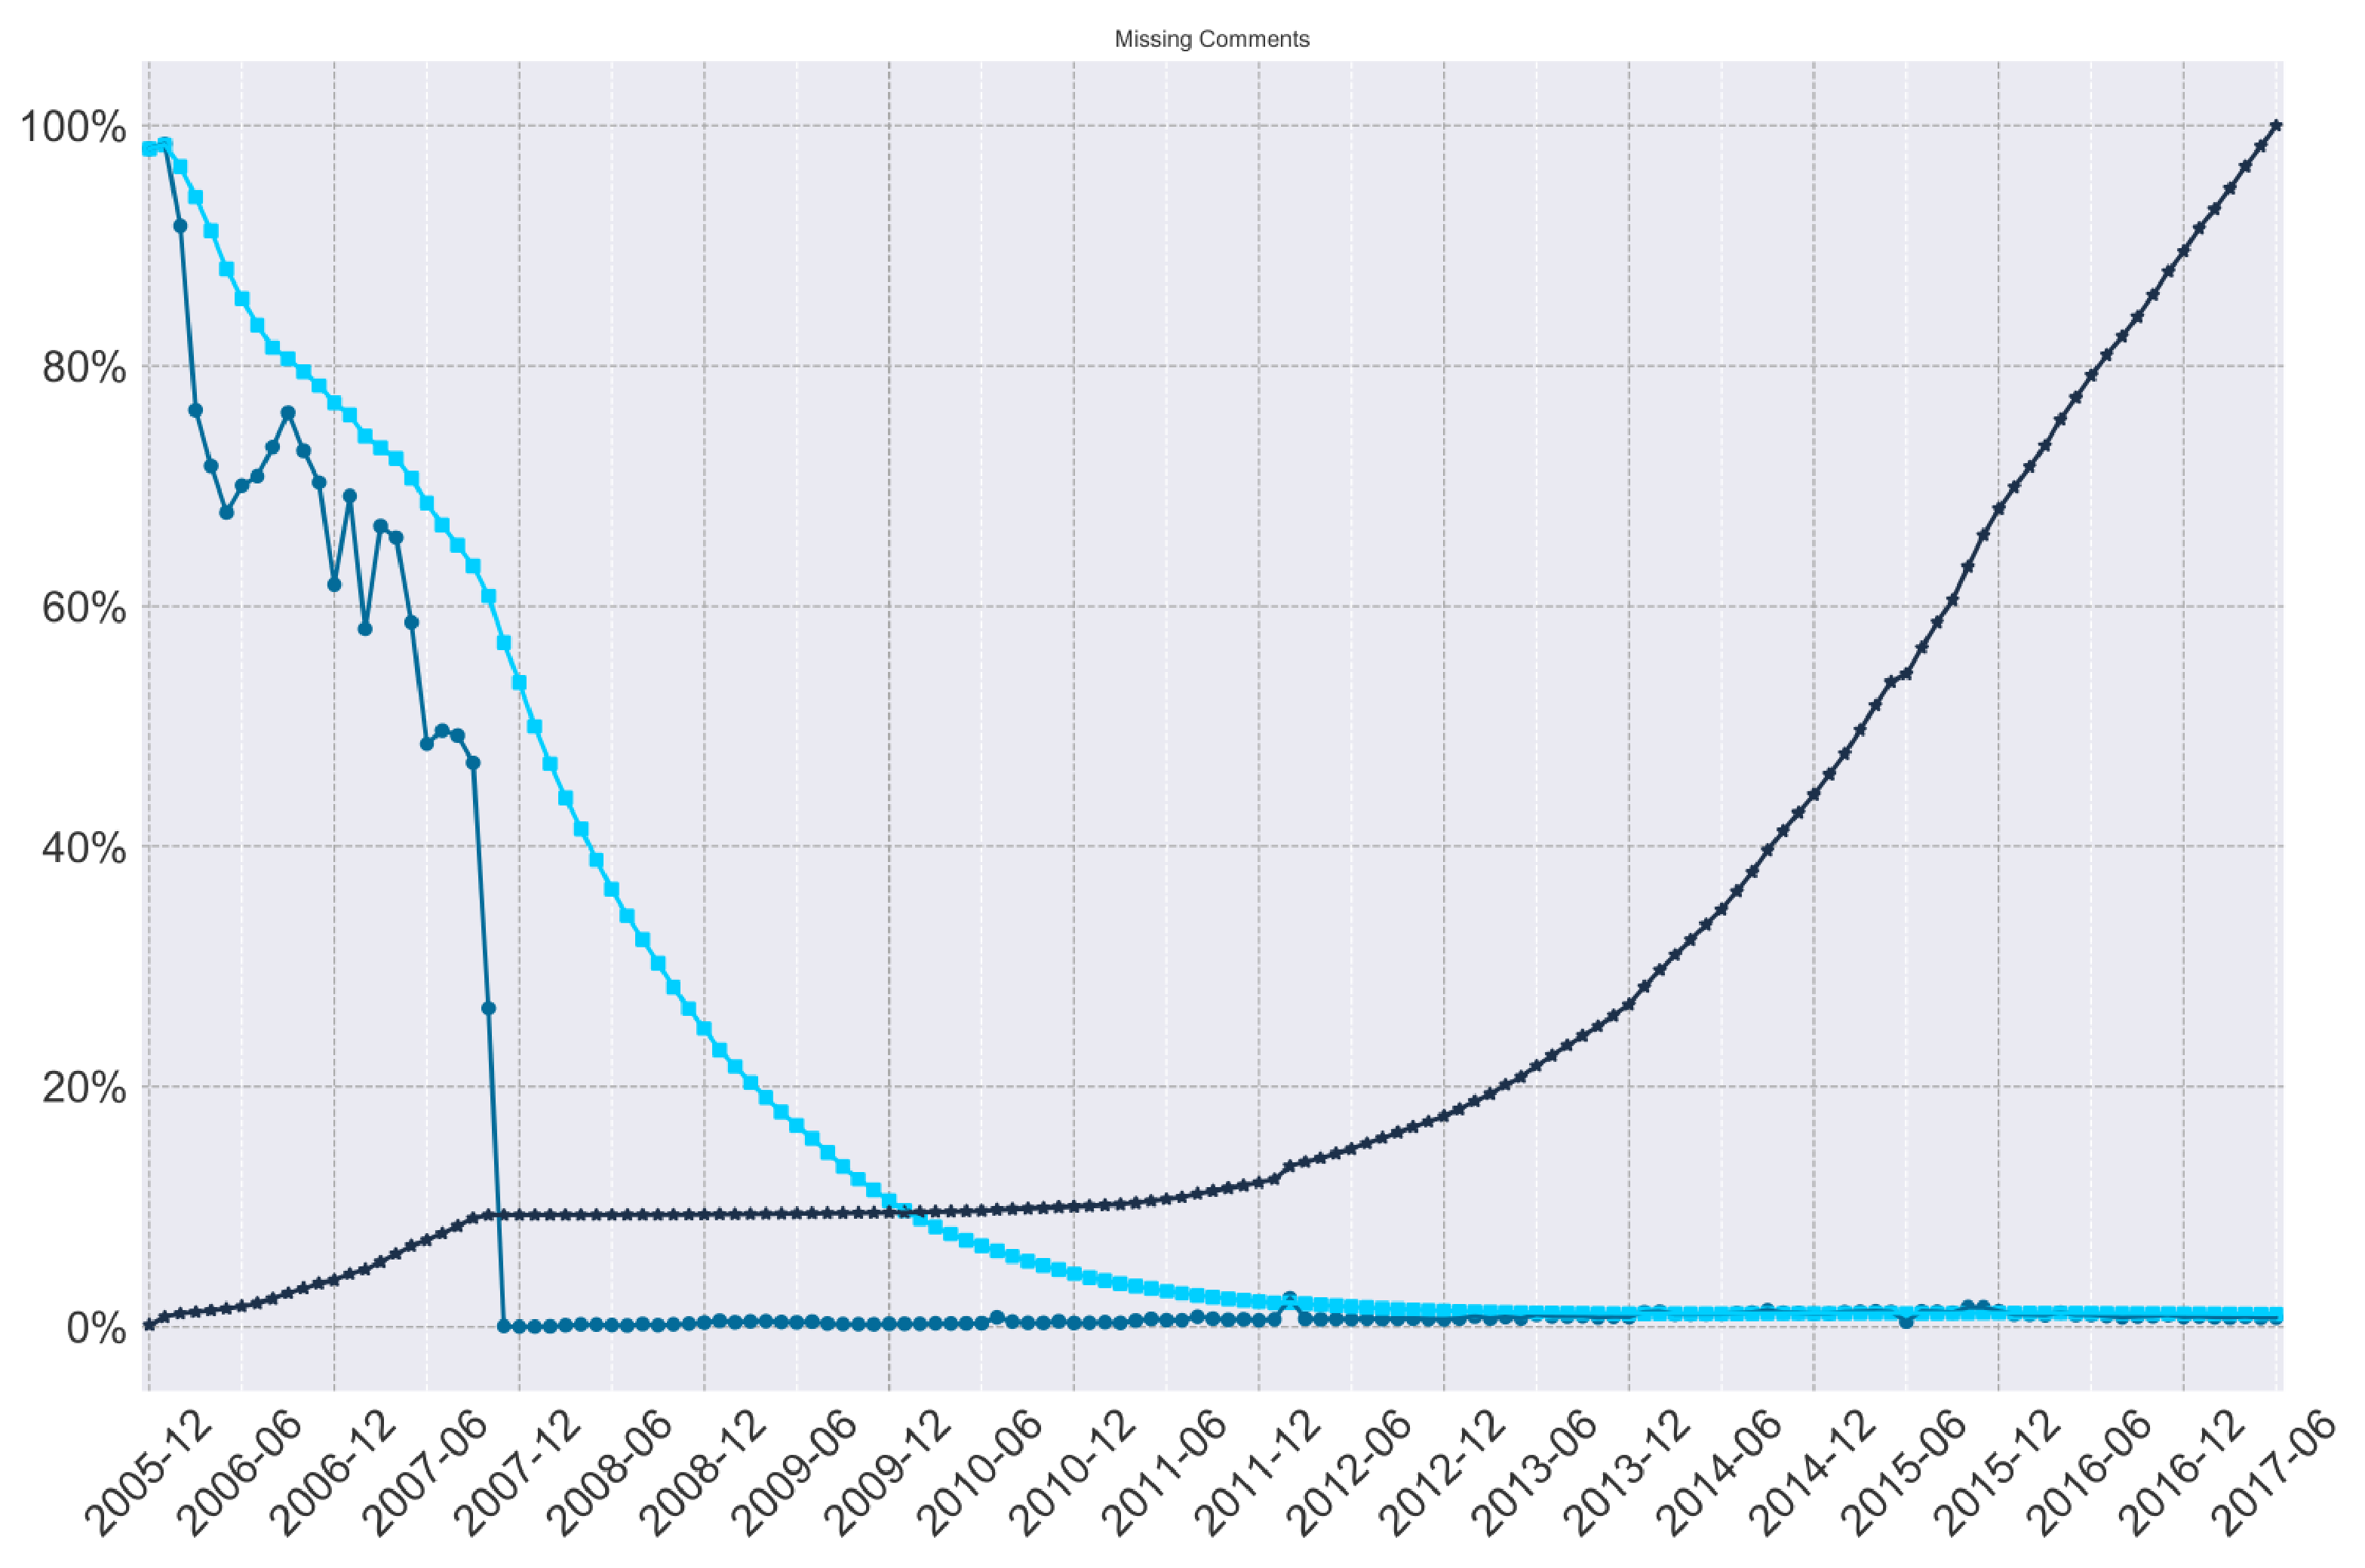
\includegraphics[width=0.8\linewidth]{./images/gaffneymatias_fig4} 

}

\caption{Anteil fehlender Kommentare. Die hellblauen Quadrate (obere
Linie) stellen den gleitenden Mittelwert fehlender Kommentare in Prozent
dar, die mittelblauen Punkte (mittlere Linie) den prozentualen Anteil
fehlender Kommentare, und die dunkelblauen Kreuze (untere Linie) die
kumulierte Gesamtzahl fehlender Kommentare \autocite[Abbildung
aus][]{Gaffney2018}}\label{fig:gf4}
\end{figure}

In Abbildung \ref{fig:gf4} stellen die mittelblauen Punkte bzw. die
anfangs mittlere der drei Linien den Anteil fehlender Kommentare in
Prozent dar. Ab April 2007 beginnt dieser Anteil zu sinken, fällt ab
etwa August 2007 stark ab und stabilisiert sich ab November 2007 im
niedrigen einstelligen Bereich. Um den Einfluss fehlender Kommentare so
gering wie möglich zu halten, setzt die Auswertung der Daten im November
2007 an und erstreckt sich bis Februar 2018.\\
Jason Baumgartner hat als Folge der Veröffentlichung von Gaffney und
Matias angekündigt, fehlende Kommentare und Beiträge nachträglich zu
erfassen \autocite{Baumgartner2018}.

\hypertarget{stichprobe}{%
\subsection{Stichprobe von Nutzern}\label{stichprobe}}

Für die angesetzte Fallstudie werden für den Beobachtungszeitraum zwei
Nutzer zufällig ausgewählt. Im Folgenden werden die Kriterien für die
Ziehung dieser Stichprobe erläutert, die aus der Verteilung der
Aktivität der Nutzer abgeleitet werden.

Für den Beobachtungszeitraum von 124 Monaten liegen etwa 3,6 Milliarden
Kommentare vor, verfasst von ca. 28 Millionen Nutzern. Für jeden dieser
Nutzer wurde bestimmt, in wie vielen Monaten er im Datensatz enthalten
ist. Diese Aktivitätsspanne reicht von nur einem Monat bis zur
Gesamtzeit von 124 Monaten. Die Hälfte der Nutzer ist zwischen einem und
sechs Monaten auf Reddit aktiv; Tabelle \ref{tab:activity-summary-full}
im Anhang enthält die wichtigsten Kennzahlen der Aktivitätsverteilung.

Stellt man diese Verteilung wie in
Abbildung~\ref{fig:age-distribution-1} als Histogramm dar, fällt die
hohe Häufung eher kurzer Aktivität auf. Abbildung
\ref{fig:age-distribution-2} wählt für dieselbe Verteilung eine
logarithmische Darstellung, die einen besseren Blick in den
\enquote{Long Tail} der Verteilung bietet. Auffällig ist bei der
logarithmischen Darstellung der Ausschlag am äußersten rechten Rand. Der
Unterschied zwischen den beiden längsten Aktivitätsklassen beträgt 382
Nutzer.

\begin{figure}

{\centering \includegraphics[width=0.8\linewidth]{thesis_files/figure-latex/age-distribution-1-1} 

}

\caption{Verteilung der Aktivität}\label{fig:age-distribution-1}
\end{figure}

\begin{figure}

{\centering \includegraphics[width=0.8\linewidth]{thesis_files/figure-latex/age-distribution-2-1} 

}

\caption{Verteilung der Aktivität, logarithmische Darstellung.}\label{fig:age-distribution-2}
\end{figure}

\begin{figure}

{\centering \includegraphics[width=0.8\linewidth]{thesis_files/figure-latex/sample-users-hist-1} 

}

\caption{Verteilung der Aktivität nach Einschränkung auf die oberen 10.000 Nutzer mit jeweils mindestens 50 Kommentaren je Monat.}\label{fig:sample-users-hist}
\end{figure}

Um sicherzustellen, dass die Historien der Nutzer möglichst frei von
Lücken sind, erfolgt die Auswahl aus den 10.000 am längsten aktiven
Nutzern. Diese müssen zudem über ihren Aktivitätszeitraum hinweg pro
Monat mindestens 50 Kommentare erstellt haben, um aussagekräftige
Interaktionsgraphen generieren zu können. Abbildung
\ref{fig:sample-users-hist} zeigt die dadurch erhaltene Verteilung der
Aktivitätsklassen als Histogramm. Die kleinste Aktivitätsspanne in
dieser neuen Verteilung liegt bei 103 Monaten. Dies entspricht einer
Überschneidung mit dem gesamten Untersuchungszeitraum zu ca. 83\%; die
Kennzahlen dieser Verteilung sind Tabelle~\ref{tab:activity-summary-cut}
im Anhang zu entnehmen.\\
Da eine Analyse aller in dieser Stichprobe enthaltenen Nutzer aus
Zeitgründen nicht möglich war, wurden exemplarisch zwei Nutzer zufällig
ausgewählt und in einer Fallstudie näher betrachtet.

\hypertarget{meth-lda}{%
\subsection{Topic-Modelle}\label{meth-lda}}

Um zu einer Zuordnung von Subreddits zu Themenkomplexen zu gelangen,
wird mittels Latent Dirichlet Allocation ein Topic-Modell erstellt und
ausgewertet. Dadurch können Communities, die ähnliches Vokabular
benutzen, unter einem Topic zusammengefasst werden.

\hypertarget{korpus}{%
\paragraph{Korpus}\label{korpus}}

Für alle Nutzer, deren Aktivität über dem Gesamtdurchschnitt von 6.67
Monaten liegt, werden die Subreddits erfasst, in denen sie Kommentare
erstellen. Durch diese Einschränkung wird verhindert, dass Subreddits in
das Topic-Modell eingehen, die ausschließlich von Nutzern aufgesucht
werden, die die Plattform nach kurzer Aktivität verlassen.

Für diese Subreddits wurden über die Reddit-API jeweils maximal 50
Beiträge aus dem Listing \enquote{Top} abgerufen. Dieses Listing liefert
eine Sortierung der Beiträge mit der besten Gesamtwertung
(\emph{Score}), also der Differenz aus Up- und Downvotes
\autocite{RedditSrc}. In der Folge erhält man so diejenigen Beiträge,
die von der Community am besten bewertet wurden. In dieser Arbeit wird
davon ausgegangen, dass ein Beitrag mit hohem Score auch repräsentativ
für die Inhalte der Community ist.

Die Titel der abgerufenen Beiträge wurden konkateniert, zu
Kleinbuchstaben normalisiert, Satzzeichen und Ziffern sowie redundante
Leerzeichen entfernt; Stoppwörter wurden nicht entfernt und
Zeichenketten mit weniger als 300 Zeichen verworfen. Damit entspricht
jedes Subreddit einem Dokument, dessen Inhalt die Titel der Top-Beiträge
bilden. Die so aufbereiteten 207.056 Dokumente bilden den Eingabe-Korpus
für ein LDA-Modell.

\hypertarget{topicverteilung}{%
\paragraph{Verteilung der Topics}\label{topicverteilung}}

Der Algorithmus zur Erstellung eines LDA-Modells ist parametrisiert
durch die Zahl der zu bestimmenden Topics \(k\) sowie der Dichte der
Topic-Wort- (Parameter \(\beta\)) bzw. der Dokument-Topic-Verteilung
(Parameter \(\alpha\)). Die beiden Parameter \(\alpha\) und \(\beta\)
werden üblicherweise so gewählt, dass die entstehenden Verteilungen dünn
besetzt sind, also Dokumente aus wenigen Topics und Topics aus wenigen
Wörtern bestehen. Der optimale Wert für \(k\) variiert zwischen
verschiedenen Korpora und lässt sich empirisch ermitteln. Wegen der
hohen Zahl an Dokumenten und damit einhergehenden Zeitaufwands wurde
dies jedoch unterlassen und stattdessen \(k = 256\) gewählt. Ob sich
diese Zahl an Topics für die betrachteten Subreddits bzw. Reddit
allgemein in der Nähe eines Optimums befindet, bleibt zu klären. Die
Start-Parameter des Algorithmus sind in Tabelle~\ref{tab:lda-params} im
Anhang aufgeführt.

Latent Dirichlet Allocation beruht auf der Annahme, dass jedes Dokument
aus verschiedenen latenten Themen zusammengesetzt wird. Das Modell
liefert für jedes Dokument eine Wahrscheinlichkeitsverteilung über die
zu bestimmenden Topics. Für die weitere Analyse in dieser Arbeit wird
aus dieser Verteilung von Topic-Wahrscheinlichkeiten eine Zuordnung von
Subreddits zu Topics abgeleitet, indem für jedes Dokument das Topic als
charakteristisch angesehen wird, dem der Algorithmus die höchste
Wahrscheinlichkeit zuweist.






\begin{figure}

{\centering \includegraphics[width=0.8\linewidth]{thesis_files/figure-latex/topic-assignments-total-1} 

}

\caption{Anzahl der Zuordnungen von Subreddits
zu Topics. Jede Säule entlang der x-Achse entspricht einem der 256
Topics. Hervorgehoben sind die 10 größten Topics mit den meisten
Zuordnungen.}\label{fig:topic-assignments-total}
\end{figure}

Abbildung \ref{fig:topic-assignments-total} stellt die Zuordnung von
Subreddits zu Topics als Histogramm dar. Auf einen großen Teil der
Topics entfallen vergleichsweise wenig Subreddits: der Hälfte aller
Topics sind weniger als neun Subreddits zugeordnet (Median: 9), das
obere Quartil liegt bei 97.5 Subreddits, das Maximum bei 45.577;
Tabelle~\ref{tab:topic-assignments-summary} im Anhang enthält die
Kennzahlen dieser Verteilung. Offensichtlich gibt es zusätzlich zu
großen bis sehr großen Topics auch eine hohe Anzahl an Nischenthemen mit
weniger als 100 zugeordneten Subreddits.







\hypertarget{interaktionsgraphen}{%
\subsection{Interaktionsgraphen aus
Kommentaren}\label{interaktionsgraphen}}

Die Kommentarverläufe von Reddit lassen sich als Interaktionsgraphen
modellieren. Jeder Knoten in einem solchen Graph stellt einen Akteur in
einem sozialen Netzwerk dar. Zwischen Akteuren manifestieren sich
gerichtete Kanten, wenn sie miteinander interagieren, in diesem Fall in
Form von Kommentaren auf Reddit. Die Richtung der Kanten gibt dabei an,
welcher Nutzer den Kommentar verfasst hat (Quelle) bzw. an welchen
Nutzer der Kommentar gerichtet ist (Senke). Im Datensatz sind Kanten
über die Beziehung zwischen den \emph{id}- bzw.
\emph{parent\_id}-Attributen realisiert. Seien dazu \(U, V\) Akteure im
sozialen Netzwerk und \(K_U, K_V\) von \(U\) resp. \(V\) verfasste
Reddit-Kommentare. Zwischen \(U\) und \(V\) wird eine gerichtete Kante
\((u,v)\) eingefügt, wenn gilt: \(K_{U}.parent\_id = K_{V}.id\).\\
Da mehrere Interaktionen zwischen denselben Partnern möglich und erlaubt
sind, handelt es sich bei den hier verwendeten Interaktionsgraphen um
Multigraphen. Da ausgehend von einem Nutzer dessen unmittelbare Kontakte
erfasst werden, spricht man hier zudem von egozentrischen Netzwerken.
Dabei ist zu beachten, dass abweichend von gängigen Definitionen des
Begriffs (etwa \autocite[S. 42]{Wasserman1994}, \autocite{Wolf2010}) in
dieser Arbeit keine Strukturen zwischen den Alteri erfasst werden,
sondern nur zwischen Ego und Alteri.

Für die beiden in Abschnitt \ref{stichprobe} ausgewählten Nutzer werden
monatliche Interaktionsgraphen erstellt. Da diese einen zeitlich
abgegrenzten Ausschnitt aus dem gesamten sozialen Netzwerk eines Nutzers
darstellen, werden sie im Folgenden auch als Snapshot-Graphen
bezeichnet.

\hypertarget{software}{%
\subsection{Verwendete Software}\label{software}}

Um die Inhalte der Subreddits über die Reddit-API abzurufen, wurde die
Python-Bibliothek \emph{PRAW}~\autocite{PRAW} verwendet, ein API-Client
speziell für Reddit.\\
Die Vorbereitung der Textkorpora für die Topic-Analyse wurde mit dem
Text-Mining-Package \emph{tm}~\autocite{R-tm} in R realisiert.\\
Für die LDA selbst wurde wegen der hohen Zahl an Inhalten eine
effiziente Implementierung benötigt, die in akzeptabler Zeit ein
Topic-Model berechnet. Die Wahl fiel dabei auf
\emph{GLDA}~\autocite{Lu2013}, das sich die hohe Rechenleistung moderner
Grafikkarten zunutze machen kann; die Software stellt eine
Weiterentwicklung von \emph{GibbsLDA++}~\autocite{Phan2007} dar.\\
Die Datenanalyse erfolgt in R mit einschlägigen Bibliotheken,
größtenteils aus dem \emph{tidyverse}~\autocite{R-tidyverse};
Visualisierungen wurden mit \emph{ggplot2}~\autocite{R-ggplot2}
erstellt.\\
Die Modellierung der Interaktionsgraphen wurde mit der R-Bibliothek
\emph{igraph}~\autocite{R-igraph} realisiert, die neben der Konstruktion
auch Funktionalität zur Analyse von Netzwerken bietet.\\
Die Arbeit selbst wurde mit \emph{bookdown}~\autocite{R-bookdown}
angefertigt, das es ermöglicht, Dokumente im Markdown-Format zu
verfassen, Codeblöcke im Text zu definieren und deren Ausgabe direkt in
den Text zu integrieren.

\clearpage

\hypertarget{datenanalyse}{%
\section{Datenanalyse}\label{datenanalyse}}

Nachdem in dem vorangehenden Teil des Kapitels die Forschungsmethodik
dargelegt wurde, widmet sich dieser Teil einer Darstellung der
Ergebnisse. Im ersten Abschnitt wird das erstellte Topic-Modell
analysiert, der zweite Teil präsentiert die Ergebnisse der Fallstudie.

\hypertarget{topic-analyse}{%
\subsection{Topic-Analyse}\label{topic-analyse}}

Aus den populärsten Beitragstiteln von Subreddits wurde mittels Latent
Dirichlet Allocation ein Topic-Modell mit 256 Topics erstellt. In
Kapitel~\ref{topicverteilung} wurde bereits auf die Verteilung der
Zuordnung von Subreddits zu Topics eingegangen; dieser Abschnitt
betrachtet die gefundenen Topics genauer.

Das LDA-Modell liefert nicht nur für jedes Dokument eine Verteilung von
Topics, sondern auch zu jedem Topic eine Wahrscheinlichkeitsverteilung
von Wörtern, die Topic-Wort-Verteilung. Sortiert man diese Häufigkeiten
absteigend, erhält man die für dieses Topic charakteristischen
Begriffe.\\
Bei einer ersten Analyse dieser Wort-Zuordnungen fiel auf, dass die
\enquote{größten} Topics\footnote{\enquote{Größe} ist hier bezogen auf
  die Zahl der einem Topic zugeordneten Subreddits, vgl.
  Kapitel~@(topicverteilung)} in den vordersten Rängen nahezu
ausschließlich Stoppwörter enthielten. Als \emph{Stoppwort} werden
Wörter bezeichnet, die in einem Dokument besonders häufig auftreten und
hauptsächlich grammatikalische Funktion besitzen, allerdings wenig
Information über den Inhalt eines Dokuments tragen. Dazu zählen etwa
bestimmte und unbestimmte Artikel, Konjunktionen und Präpositionen.\\
Tabelle \ref{tab:topics-with-stopwords} enthält eine Aufstellung der
häufigsten Wörter für die vier größten Subreddits.





\begin{table}

\caption{\label{tab:topics-with-stopwords}Häufigste Wörter der vier größten
LDA-Topics. Die Spalten enthalten die Topic-ID, die Anzahl zugeordneter
Subreddits \emph{n} sowie die 15 häufigsten Wörter.}
\centering
\begin{tabular}[t]{crl}
\toprule
Topic & n & Wörter\\
\midrule
235 & 45.577 & the, a, to, i, is, you, this, of, and, in, it, that, on, for, when\\
122 & 34.240 & to, a, for, the, and, i, you, is, of, in, how, on, what, with, this\\
69 & 18.504 & my, a, i, the, this, of, and, to, in, for, on, it, from, is, with\\
194 & 13.146 & the, to, for, of, on, and, new, is, in, a, now, we, at, with, this\\
\bottomrule
\end{tabular}
\end{table}

Diese Verteilung ist wenig informativ in Bezug auf den Inhalt der
Topics. Vielmehr lässt sich hier erkennen, dass eine große Zahl von
Subreddits durch Inhalte geprägt ist, die sich nicht durch Schlagworte
voneinander abgrenzen lassen. Es sei darauf hingewiesen, dass sich auch
in klarer definierten Topics Stoppwörter in den vorderen Rängen finden,
allerdings in Nachbarschaft durchaus informativer Begriffe; die
häufigsten fünf Wörter für Topic 131 (1.166 Subreddits) etwa sind
\enquote{food, and, with, chicken, recipe}, was auf einen Bezug zum
Thema \enquote{Essen} bzw. \enquote{Kochen} schließen lässt.

In der Nachbereitung des Topic-Modells wurde aus der
Wort-Topic-Verteilung eine Liste an Stoppwörtern der englischen Sprache
entfernt; diese Liste entstammt dem R-Package \emph{tm}~\autocite{R-tm}.
Damit gelang es, auch diese initial wenig aussagekräftigen Topics in
Ansätzen zu charakterisieren. Eine Auswahl aussagekräftiger Wörter zeigt
Tabelle \ref{tab:topics-without-stopwords}, und Tabelle
\ref{tab:app-top-words-tab} im Anhang enthält für alle Topics, denen
mindestens 500 Subreddits zugeordnet wurden, die 25 häufigsten Wörter.






\begin{table}

\caption{\label{tab:topics-without-stopwords}Häufigste Wörter der vier größten
Subreddits, analog zu Tabelle \ref{tab:topics-with-stopwords}.
Dargestellt ist lediglich eine Auswahl charakteristischer Begriffe,
deren Ordnung untereinander jedoch beibehalten wurde.}
\centering
\begin{tabular}[t]{cr >{\raggedright\arraybackslash}p{0.8\textwidth}}
\toprule
Topic & n & Wörter\\
\midrule
235 & 45.577 & like, just, one, people, subreddit, sub, go, see\\
122 & 34.240 & help, can, anyone, need, know, please, just, best, question, people\\
69 & 18.504 & first, just, new, got, made, one, today, like, day, im, time, love, found, happy, finally, good\\
194 & 13.146 & new, now, will, update, first, official, th, news, us, coming, next, live, video, available, today, time, release, team\\
\bottomrule
\end{tabular}
\end{table}

Bei der Analyse der größten Topics fällt auf, dass sich auch nach
Entfernung der Stoppwörter nur schwer über einzelne Wörter auf die
thematische Ausrichtung schließen lässt. Betrachtet man jedoch die
Wörter in ihrem Kontext, zeichnen sich erste Tendenzen ab. In Topic 235
etwa stehen Begriffe wie \enquote{subreddit} und \enquote{sub} in
Nachbarschaft von \enquote{like}, \enquote{go} und \enquote{see};
vermutlich ist dieses Topic stark von der Autoreferentialität von Reddit
geprägt, ein Umstand, auf den in der Diskussion der Ergebnisse in
Kapitel~\ref{diskussion} noch näher eingegangen wird.\\
Ähnlich verhält es sich mit den übrigen Topics, die hier angesprochen
wurden: Topic 122 scheint sich mit Gesuchen nach Hilfe bzw. Ratschlägen
zu befassen (\enquote{can}, \enquote{anyone}, \enquote{need},
\enquote{know}, \enquote{question}), Topic 69 mit Berichten über
positive Ereignisse bzw. Errungenschaften (\enquote{first},
\enquote{new}, \enquote{today}, \enquote{got}, \enquote{made},
\enquote{love}, \enquote{finally}), und Topic 194 schließlich scheint
sich mit offiziellen Bekanntmachungen zu beschäftigen (\enquote{new},
\enquote{now}, \enquote{update}, \enquote{official}, \enquote{news},
\enquote{release}, \enquote{team}). Trotz dieser Erkenntnisse bleiben
diese Topics einigermaßen schwierig einzuordnen, zumal sich erst in der
nachträglichen Bearbeitung \enquote{echte} Topics
herauskristallisierten.

Abschließend sei auf einige interessante Topics hingewiesen, die sich
aus Tabelle \ref{tab:app-top-words-tab} im Anhang ablesen lassen. Topic
210 lässt wenig Zweifel an politischen Ausrichtung des Inhalts, mit
Schwerpunkt auf US-amerikanischen Themen (\enquote{trump},
\enquote{president}, \enquote{donald}, \enquote{bill},
\enquote{american}).\\
Eine allgemein wissenschaftliche Ausrichtung lässt sich bei Topic 219
vermuten, mit Begriffen wie \enquote{science}, \enquote{research},
\enquote{theory} und \enquote{study}.\\
Wörter wie \enquote{google}, \enquote{windows}, \enquote{app},
\enquote{code}, \enquote{tutorial} und \enquote{programming}
kennzeichnen Topic 239; vermutlich handelt es sich um IT-Themen, mit
einem erkennbaren Schwerpunkt auf Softwareentwicklung (\enquote{code},
\enquote{source}, \enquote{open}).\\
Auffällig sind schließlich auch die Topics 46, 72 und 217, die
ausschließlich spanische, deutsche resp. französische Wörter enthalten
-- im Falle des Französischen gar Interpunktion in Form schließender
Guillemets (\guillemotleft). Obgleich es sich um Stoppwörter handelt,
lassen sich hinter diesen Topics eigene Sprach-Communities vermuten.

Ohne diese Analyse zu tief geraten zu lassen, lässt sich festhalten,
dass die Topics des erstellten LDA-Modells hinreichend gut
abgeschlossene Themenkomplexe identifiziert haben, die man auch in einem
OSN wie Reddit vermuten würde: Hilfe/Selbsthilfe, Selbstdarstellung,
Politik, Wissenschaft und Technik, sowie individuelle Communities, die
in ihrer Landessprache kommunizieren. Dies alles ist umso
bemerkenswerter, als dass es sich hier \enquote{nur} um ein mit
statistischen Methoden erstelltes Modell menschlicher Sprache handelt,
das überdies keine Kenntnis über die Themenverteilung besitzt.

\hypertarget{fallstudie}{%
\subsection{Fallstudie}\label{fallstudie}}

Die folgenden drei Abschnitte befassen sich jeweils mit einem
individuellen Nutzer, der aus dem Long Tail der Aktivitätsverteilung für
Nutzer gezogen wurde. Für alle drei wurde die Themenhistorie über den
gesamten Untersuchungszeitraum von November 2007 bis Februar 2018
erstellt, ebenso wie die zugehörigen Interaktionsgraphen, in denen die
Kommunikation mit anderen Nutzern abgebildet ist.

\hypertarget{monocasa}{%
\subsubsection{monocasa}\label{monocasa}}

\FloatBarrier

Der Nutzer mit dem Namen \enquote{monocasa} ist im betrachteten
Ausschnitt aus dem Datensatz in 119 Monaten enthalten und hat insgesamt
7.996 Kommentare erstellt, was im Mittel 67,19 Kommentaren pro Monat
entspricht.

\hypertarget{topic-verteilungen}{%
\paragraph{Topic-Verteilungen}\label{topic-verteilungen}}

Um einen Überblick zu erhalten, in welchen Topics der Nutzer aktiv ist,
bietet es sich an, die Verteilung der Kommentare zu visualisieren. Alle
Kommentare werden über das Subreddit, in dem sie erstellt wurden, einem
Topic zugeordnet. In Abbildung \ref{fig:monocasa-topic-distribution} ist
zu erkennen, dass der Nutzer hauptsächlich in drei Topics aktiv ist:
210, 239 und 235. Auch der zeitliche Verlauf der Topics in Abbildung
\ref{fig:monocasa-area-chart-comms-full} lässt dies erkennen. Wie
bereits weiter oben festgestellt, handelt es sich bei Topic 239 um
technisch orientierte Inhalte, bei 210 um Politik mit Schwerpunkt auf
US-amerikanischen Themen; Topic 235 wurde als Reddit-selbstreferentiell
identifiziert. Die weitere Analyse wird sich vor allem auf diese großen
Topics stützen, da sie die meiste Aktivität des Nutzers auf sich
vereinen.




\begin{figure}

{\centering \includegraphics[width=0.8\linewidth]{thesis_files/figure-latex/monocasa-topic-distribution-1} 

}

\caption{Verteilung von Kommentaren über
Topics.}\label{fig:monocasa-topic-distribution}
\end{figure}

Bei der Analyse des Topic-Verlaufs fällt auf, dass der Anteil von Topic
239 zwischen 2013 und 2014 zweimal stark abfällt: einmal im Juli 2013
und kurz darauf im Oktober 2013. Fällt der Anteil eines Topics auf 0
wird dies im weiteren Verlauf dieser Analyse gleichgesetzt mit einem
Verlassen dieser thematischen Community. Im Folgenden wird der Frage
nachgegangen, was für dieses Verlassen ursächlich sein könnte. Dazu
werden verschiedene Eigenschaften der Topic-Verläufe sowie der lokalen
Ego-Netzwerke des Nutzers herangezogen. Der Untersuchungszeitraum wird
auf die Zeit zwei Jahre vor und zwei Jahre nach dem Verlassen im Oktober
2013 festgelegt; dies ist durch die beiden gepunkteten Linien in
Abb.~\ref{fig:monocasa-area-chart-comms-full} angedeutet.

Auch für die Alteri lässt sich ein ähnlicher Topic-Verlauf bestimmen,
indem pro Monat für jeden von ihnen das Topic bestimmt wird, in dem er
die meisten Kommentare verfasst; so wird jeder dieser Nutzer auf ein
einzelnes Topic festgelegt, das ihn charakterisiert. Damit lässt sich
bestimmen, welchen Anteil ein Topic unter den Alteri ausmacht. Abbildung
\ref{fig:monocasa-area-chart-alters-full} lässt erkennen, dass in dem
gewählten Zeitraum der Anteil der Alteri, die sich ebenfalls an diesem
Topic beteiligen, auf 0 sinkt. Zudem fällt auf, dass sich Ego und Alteri
durchaus in ihren Interessen überschneiden; in zwölf Topics erstellen
sowohl Ego als auch Alteri Kommentare.





\begin{figure}

{\centering \includegraphics[width=0.8\linewidth]{thesis_files/figure-latex/monocasa-area-chart-comms-full-1} 

}

\caption{Topic-Verteilung von Egos
Kommentaren. Dargestellt sind die relativen Anteile eines Topics an
allen Kommentaren, die Ego in einem gegebenen Monat erstellt.}\label{fig:monocasa-area-chart-comms-full}
\end{figure}





\begin{figure}

{\centering \includegraphics[width=0.8\linewidth]{thesis_files/figure-latex/monocasa-area-chart-alters-full-1} 

}

\caption{Topic-Verteilung der Alteri im
lokalen Netzwerk. Dargestellt ist der Anteil der Alteri, deren
Hauptinteresse in dem jeweiligen Monat dem dargestellten Topic gilt.}\label{fig:monocasa-area-chart-alters-full}
\end{figure}

\hypertarget{zusammenhang-zwischen-ego-und-alteri}{%
\paragraph{Zusammenhang zwischen Ego und
Alteri}\label{zusammenhang-zwischen-ego-und-alteri}}

Zunächst soll betrachtet werden, wie das Kommentar-Verhalten von Ego mit
der Zusammensetzung seiner Alteri zusammenhängt. Die Vermutung dabei
ist, dass ein höherer Anteil Alteri eines Topics dazu führt, dass auch
Ego vermehrt in diesem Topic aktiv ist, bzw. Ego basierend auf seinen
Interessen sein Umfeld auswählt.








\begin{figure}

{\centering \includegraphics[width=0.8\linewidth]{thesis_files/figure-latex/monocasa-prob-corr-1} 

}

\caption{Anteil Kommentare vs.~Anteil Alteri in einem
Topic. Die x-Achse zeigt den relativen Anteil Kommentare, die Ego in
einem Topic verfasst, die y-Achse den Anteil Alteri, der sich diesem
Topic hauptsächlich widmet. Spearmans \(\rho\) zeigt die Stärke der
Korrelation (\(^{*}p\le0.05\), \(^{**}p\le0.01\), \(^{***}p\le0.001\),
\(^{n.s.}\)nicht signifikant).}\label{fig:monocasa-prob-corr}
\end{figure}

Abbildung \ref{fig:monocasa-prob-corr} zeigt Streudiagramme der Anteile,
aufgeschlüsselt nach Topic. Da die berechneten Topic-Anteile nach
Shapiro-Wilk nicht normalverteilt sind, wurde zur Bestimmung der Stärke
der Korrelation Spearmans \(\rho\) verwendet. Die Korrelationen für die
beiden größeren Topics 210 und 239 fällt mittel bis stark aus und ist
signifikant auf dem 0.1\%-Niveau. Für 235 fällt die Korrelation
schwächer aus, ist aber ebenfalls signifikant. Wie vermutet lassen sich
vor allem bei den großen Topics, in denen der Nutzer vermehrt Aktivität
verzeichnet, lineare Zusammenhänge erkennen. Auffällig dabei ist, dass
die Regression der beiden Topics 210 und 239 unterhalb der Diagonalen
verläuft; der Nutzer ist scheinbar verstärkt in diesen Topics aktiv,
obwohl sein Umfeld nicht \enquote{mitzieht}.

\hypertarget{anziehungskraft-von-topics}{%
\paragraph{Anziehungskraft von
Topics}\label{anziehungskraft-von-topics}}

Was macht ein Topic attraktiv für einen Nutzer? Zum Einen sollte es ihn
selbst interessieren, zum anderen sollte aber auch sein Umfeld dieses
Thema kennen und sich ihm widmen. Um diesen Zusammenhang messbar zu
machen, wird im folgenden ein naiver Ansatz gewählt, um einen Index zu
bilden. Seien \(r_{A}\) und \(r_{C}\) die Anteile der Alteri resp.
Kommentare an einem Topic. Dann sei ihr Produkt

\begin{equation}
g = r_A r_C
\label{eq:attractivity}
\end{equation}

ein Maß für die Attraktivität bzw. Anziehungskraft eines Topics.
\eqref{eq:attractivity} wird minimal, wenn einer der beiden Faktoren 0
ist, also Ego keine Kommentare in diesem Topic erstellt oder keiner der
Alteri daran interessiert ist. Sind beide Anteile hoch, übt auch das
Topic hohe Anziehungskraft aus. Da beide Faktoren relative Anteile
darstellen, ist auch ihr Produkt dimensionslos.






\begin{figure}

{\centering \includegraphics[width=0.8\linewidth]{thesis_files/figure-latex/monocasa-interestingness-1} 

}

\caption{Attraktivität angetragen über den
zeitlichen Verlauf. Die gepunktete Linie markiert den Monat, in dem der
Nutzer Topic 239 verlässt. In dieser Darstellung enthalten sind alle
Topics, deren Attraktivität in Summe größer 0 ist.}\label{fig:monocasa-interestingness}
\end{figure}

Abbildung \ref{fig:monocasa-interestingness} zeigt die zeitliche
Entwicklung von \(g\) für den Nutzer monocasa. Es sind einige Spitzen zu
erkennen, die auf sehr hohe, aber zeitlich begrenzte Attraktivität
hindeuten. Der Zeitpunkt des Austritts aus 239 liegt inmitten einer
Phase niedriger Anziehungskraft dieses Topics.

Um die spitzen Ausschläge besser verstehen zu können, bietet es sich an,
die Gesamtzahl aller Kommentare zu betrachten.
Abbildung~\ref{fig:monocasa-total-posts} zeigt den zeitlichen Verlauf
erstellter Kommentare je Topic, sowie deren Summe. Der Knick zum
Zeitpunkt, als der Nutzer Topic 239 verlässt, deutet darauf hin, dass
hier eine Phase allgemein geringer Aktivität vorliegt, in der monocasa
generell nur wenige Kommentare verfasst.





\begin{figure}

{\centering \includegraphics[width=0.8\linewidth]{thesis_files/figure-latex/monocasa-total-posts-1} 

}

\caption{Anzahl Kommentare je Topic über die Zeit
aufgetragen, sowie die Summe aller Kommentare als rot gestrichelte
Linie.}\label{fig:monocasa-total-posts}
\end{figure}

\hypertarget{analyse-des-netzwerks}{%
\paragraph{Analyse des Netzwerks}\label{analyse-des-netzwerks}}





\begin{figure}

{\centering \includegraphics[width=0.8\linewidth]{thesis_files/figure-latex/monocasa-network-structure-1} 

}

\caption{Zahl der Knoten sowie Kanten des
lokalen sozialen Netzwerks, angetragen über die Zeit. Wie zuvor auch
kennzeichnet die gepunktete Linie den Austritt aus Topic 239.}\label{fig:monocasa-network-structure}
\end{figure}

In den vorangegangenen Abschnitten wurde die Themenhistorie der Nutzer
betrachtet. Im Folgenden wird nun der Blick auf das persönliche soziale
Netzwerk des Nutzers gerichtet. Um einen ersten Eindruck von der Größe
und Struktur der Kommunikationsbeziehungen des Nutzers zu erhalten,
zeigt Abbildung \ref{fig:monocasa-network-structure} die Anzahl der
Knoten und Kanten im sozialen Graph des Nutzers über den gesamten
Beobachtungszeitraum hinweg. Das Wachstum des Graphen ist hier gut zu
erkennen, ebenso der Zeitpunkt sehr geringer Aktivität im Oktober 2013.
Knoten und Kanten wachsen in etwa gleich stark an, woraus sich schließen
lässt, dass der Nutzer die Anzahl seiner Kontakte ausbaut.

\hypertarget{reziprozitat-1}{%
\paragraph{Reziprozität}\label{reziprozitat-1}}

Wie bereits in früheren Kapiteln erwähnt gibt ein Maß für Reziprozität
Auskunft darüber, ob Kanten zwischen Knoten wechselseitig oder
asymmetrisch angelegt sind. Als Maß für Reziprozität in sozialen
Netzwerken wählt diese Arbeit den Katz-Powell-Index (im Verlauf auch
\(\rho_{KP}\)). Dieser nimmt Werte im Bereich
\(-\infty < \rho_{KP} \le 1\) an und zeigt an, ob Kanten eher erwidert
werden (nahe 1) bzw. ob der Graph eher zu asymmetrischen Kanten tendiert
(nahe bzw. kleiner 0).




\begin{figure}

{\centering \includegraphics[width=0.8\linewidth]{thesis_files/figure-latex/monocasa-katz-powell-1} 

}

\caption{Katz-Powell-Index \(\rho_{KP}\) angetragen
über die gesamte Zeit.}\label{fig:monocasa-katz-powell}
\end{figure}

Abbildung \ref{fig:monocasa-katz-powell} zeigt, dass der Index zu Beginn
langsam ansteigt und im ersten Drittel sein vorläufiges Maximum
erreicht. Der allgemein eher hohe Wert zwischen 0.4 und 0.5 deutet
darauf hin, dass in diesem Graphen Kanten eher erwidert werden. Zu
beachten ist jedoch der starke Fall ins Negative im Oktober 2013, der
anzeigt, dass der Graph eher zu asymmetrischen Kanten neigt.

\hypertarget{thematische-teilgraphen}{%
\paragraph{Thematische Teilgraphen}\label{thematische-teilgraphen}}

Der gesamte Snapshot-Graph \(G\) des Nutzers umfasst alle Interaktionen,
die in einem Monat stattfinden. Kanten manifestieren sich von Ego zu
Alteri wenn der eine auf einen Kommentar des anderen reagiert. Für Ego
ist bekannt, in welchen fünf Topics er in einem Monat am meisten
Kommentare erstellt hat, für Alteri ist jeweils ein Topic bekannt. Sei
nun \(G'\) der Teilgraph, der entsteht, wenn man alle Kanten zu Alteri
entfernt, die kein Topic mit Ego gemeinsam haben. Die verbleibenden
Knoten sind dann Nutzer, die sich für ein Topic interessieren, in dem
auch Ego in diesem Monat aktiv ist.

In Abbildung \ref{fig:monocasa-topical-subgraph} ist für jeden der
beiden Graphen \(G\) und \(G'\) die Zahl der Knoten \(|G|\) und \(|G'|\)
sowie deren Differenz \(|G|- |G'|\) im zeitlichen Verlauf angetragen;
\(|G|\) wird auch als \emph{Ordnung} des Graphen bezeichnet. Die
Differenz der beiden Ordnungen bezeichnet hier die Menge der Knoten, die
kein thematisches Interesse mit Ego teilen. Diese Größe wird 0, wenn
alle Knoten des gesamten Graphen auch im Teilgraphen enthalten sind, die
\enquote{thematische Überdeckung} von Ego und Alteri also maximal ist.
Die Abbildung zeigt, dass die Differenz nahe 0 einsetzt, im Verlauf der
Zeit jedoch zunimmt, wenn auch langsamer als die beiden Ordnungen.
Daraus lässt sich schließen, dass der Nutzer wohl zugleich mit einer
Ausweitung seiner Interaktionen diese auch diversifiziert.






\begin{figure}

{\centering \includegraphics[width=0.8\linewidth]{thesis_files/figure-latex/monocasa-topical-subgraph-1} 

}

\caption{Ordnung des gesamten Graphen \(G\) und
des thematischen Teilgraphen \(G'\),sowie deren Differenz
\(|G| - |G|'\). Die angetragenen Regressionsgeraden verdeutlichen das
unterschiedliche Wachstum der Größen.}\label{fig:monocasa-topical-subgraph}
\end{figure}

\hypertarget{reziprozitaten-im-teilgraph}{%
\paragraph{Reziprozitäten im
Teilgraph}\label{reziprozitaten-im-teilgraph}}

Neben der Ordnung lässt sich auch die Reziprozität des thematischen
Teilgraphen bestimmen. Erneut wird dazu der Index von Katz und Powell
herangezogen. Die Konstruktion des Teilgraphen erfolgt ähnlich wie im
vorherigen Abschnitt, allerdings wird auch Ego auf das Topic festgelegt,
in dem er am aktivsten ist; nachfolgend wird dieser Teilgraph auch als
\enquote{monothematisch} bezeichnet, da nur mehr ein einzelnes Topic
enthalten ist. Dadurch kann die Frage beantwortet werden, ob Nutzer dazu
neigen, zu Gleichgesinnten eher symmetrische Beziehungen aufzubauen.

Die Vermutung liegt nahe, dass Kanten zu Gleichgesinnten eher
wechselseitig ausfallen als Kanten zu Nutzern, mit denen man keine
Interessen teilt. Um dies zu prüfen, werden für den gesamten Graph \(G\)
und den \enquote{monothematischen} Teilgraph \(G'\) die Indizes
berechnet, sowie die Differenz der beiden Größen,
\(\rho_{kp}(G')-\rho_{KP}(G)\). Diese wird umgekehrt zu der im
vorherigen Abschnitt gebildet, da vermutet wird, dass der thematische
Teilgraph höhere Indexwerte aufweist als der Gesamtgraph, und die
Differenz damit positiv bleibt, was bei der Interpretation hilft.
Abbildung \ref{fig:monocasa-topical-subgraph-reciprocity} bestätigt die
Vermutung in Teilen. Der Index nimmt für den Teilgraphen tatsächlich
häufig höhere Werte an, dieser tendiert also eher zu wechselseitigen
Kanten; allerdings kehrt sich der Index auch ins Negative und oszilliert
um die 0. Bemerkenswert ist das Loch im Oktober 2013, das dadurch zu
erklären ist, dass für den Index an dieser Stelle kein sinnvoller Wert
berechnet werden kann, da der Graph, für den er bestimmt werden soll,
leer ist. In diesem Kontext enthält also der Teilgraph, in dem alle
Knoten dasselbe Topic haben wie Ego, gar keine Knoten -- Ego hat in
diesem Monat keine Alteri, die sein Interesse teilen.









\begin{figure}

{\centering \includegraphics[width=0.8\linewidth]{thesis_files/figure-latex/monocasa-topical-subgraph-reciprocity-1} 

}

\caption{Index von Katz und Powell
für den monothematischen Teilgraphen der entsteht, wenn man Ego und
Alteri auf ihr aktivstes Topic reduziert und nur Kanten zwischen Nutzern
mit gleichen Topics zulässt. Ebenfalls dargestellt ist die Differenz der
beiden Größen, die 0 wird, wenn beide Graphen gleich reziprok sind,
gegen -1 geht wenn der Gesamtgraph eher wechselseitig und gegen +1 wenn
der Teilgraph eher symmetrisch angelegt ist.}\label{fig:monocasa-topical-subgraph-reciprocity}
\end{figure}

\hypertarget{groe-der-teilgraphen}{%
\paragraph{Größe der Teilgraphen}\label{groe-der-teilgraphen}}

Die abschließende Betrachtung gilt der Anzahl an Knoten und Kanten in
den jeweiligen Teilgraphen. Mittels der Zahl der Knoten kann
festgestellt werden, mit wie vielen Alteri der Nutzer kommuniziert, die
Zahl der Kanten gibt Aufschluss darüber, wie viele Interaktionen
stattfinden. Abbildung \ref{fig:monocasa-subgraph-per-topic} zeigt diese
beiden Maße für jedes Topic, in Abbildung
\ref{fig:monocasa-subgraph-one-topic} wird speziell Topic 239 in den
Fokus gerückt.




\begin{figure}

{\centering \includegraphics[width=0.8\linewidth]{thesis_files/figure-latex/monocasa-subgraph-per-topic-1} 

}

\caption{Verteilung der Knoten und Kanten in
den thematischen Teilgraphen.}\label{fig:monocasa-subgraph-per-topic}
\end{figure}




\begin{figure}

{\centering \includegraphics[width=0.8\linewidth]{thesis_files/figure-latex/monocasa-subgraph-one-topic-1} 

}

\caption{Verteilung der Knoten und Kanten im
thematischen Teilgraphen von Topic 239.}\label{fig:monocasa-subgraph-one-topic}
\end{figure}

Die Verteilung der Kanten in Abbildung
\ref{fig:monocasa-subgraph-one-topic} weist in den Monaten vor dem
Verlassen im Oktober 2013 vergleichsweise viele Kanten zu wenigen Knoten
auf. Hier könnte ein Indiz für den \enquote{Bruch}mit diesem Topic
liegen, zumal sich diese Beobachtung im Juni 2014 wiederholt. So ist es
denkbar, dass der Nutzer einen regen Austausch mit wenigen
Einzelpersonen erlebt hat, der ihn dazu veranlasst hat, dieses Topic in
der Folge zu meiden. Ebenso denkbar ist es aber auch, dass externe
Gründe aus der physischen Welt dafür verantwortlich sind, etwa ein
Urlaub oder ein Umzug. Klar ist, dass an dieser Stelle keine definitive
Antwort gegeben werden kann, und dass weitere Methoden herangezogen
werden müssen, um diese Frage zu klären.

\hypertarget{cavedave}{%
\subsubsection{cavedave}\label{cavedave}}

\FloatBarrier

Im vorherigen Kapitel wurde exemplarisch für einen Nutzer eine Analyse
der Topic-Historie sowie der Interaktionsgraphen unternommen. Die dort
unternommenen Gedankengänge werden hier für einen weiteren Nutzer
fortgeführt.

\hypertarget{zahl-der-kommentare}{%
\paragraph{Zahl der Kommentare}\label{zahl-der-kommentare}}

Der Nutzer \enquote{cavedave} ist im Datensatz über den gesamten
zeitlichen Verlauf von 124 Monaten enthalten. Er hat insgesamt 7.734
Kommentare erstellt, also 62,37 im monatlichen Mittel.






\begin{figure}

{\centering \includegraphics[width=0.8\linewidth]{thesis_files/figure-latex/cavedave-total-posts-1} 

}

\caption{Anzahl Kommentare je Topic über die Zeit
aufgetragen. Dargestellt sind LOESS-Regressionen über die Zahl der je
Monat erstellten Kommentare; die gestrichelte rote Linie stellt die
Summe aller Kommentare eines Monats dar.}\label{fig:cavedave-total-posts}
\end{figure}

Die Dynamik des Kommentarverhaltens zeigt Abbildung
\ref{fig:cavedave-total-posts}. Die Summe aller in einem Monat
erstellten Kommentare (rot gestrichelte Linie) fällt bereits, als der
Beobachtungszeitraum einsetzt. Sie besitzt zudem mehrere lokale Minima
und Maxima sowie zu Beginn des Jahres 2013 ein globales Minimum; das
globale Maximum erreicht sie am äußersten rechten Rand, dem Ende des
Untersuchungszeitraums im Februar 2018.\\
Unterhalb der Linie, die die Summe aller Kommentare abbildet, sind die
Topics im Einzelnen aufgeschlüsselt. Hier zeigt sich, dass auch
innerhalb der Topics eine gewisse Fluktuation herrscht. So fällt etwa
die dunkelrote Linie, die Topic 239 darstellt, ebenfalls am Beginn des
Zeitraums und verlässt im weiteren Verlauf den Bereich um die 0 nicht
mehr. Hervorzuheben ist auch die Kreuzung der beiden Linien für Topic
219 und 235 um den Beginn des Jahres 2013 herum. Während cavedave
weniger Kommentare in Topic 219 verfasst, nimmt seine Aktivität in 235
allmählich zu und erreicht ab Mitte 2013 sogar das einstweilige Maximum
im Vergleich zu allen anderen Topics. Es sieht so aus, als
\enquote{rette} Topic 235 noch einmal die allgemein fallende Tendenz,
auf Reddit Kommentare zu erstellen.\\
Im weiteren Verlauf wird daher ein besonderer Fokus auf den Zeitraum
zwischen Januar 2012 und Januar 2014 gelegt, da sich hier die größte
Dynamik im Kommentarverhalten zeigt. Anders als bei der vorherigen
Betrachtung von monocasa wird hier der Beobachtungszeitraum nicht weiter
eingeschränkt.

\hypertarget{verteilung-der-kommentare}{%
\paragraph{Verteilung der Kommentare}\label{verteilung-der-kommentare}}




\begin{figure}

{\centering \includegraphics[width=0.8\linewidth]{thesis_files/figure-latex/cavedave-topic-distribution-1} 

}

\caption{Verteilung von Kommentaren über
Topics.}\label{fig:cavedave-topic-distribution}
\end{figure}

Eine Sicht auf die Verteilung innerhalb der Topics bietet Abbildung
\ref{fig:cavedave-topic-distribution}. Nochmals deutlicher als in der
vorherigen Abbildung treten hier die Topics 210, 219 und 235 als
Hauptinteresse des Nutzers hervor. Bei allen drei liegt der Median um
12,5 Kommentare, die Extrema von 219 und 235 übersteigen mit 86 bzw. 119
Kommentaren deutlich das monatliche Mittel von 62,37. Allerdings ist
darauf zu achten, dass Inhalte von Topic 235 hauptsächlich auf Reddit
selbst bezogen zu sein scheinen; dies macht eine Analyse von
Nutzerinteressen schwierig, da nicht erkennbar ist, was hier konkret
thematisiert wird. Die beiden anderen Topics lassen sich in ihrer
Ausrichtung deutlich trennschärfer als politisch (210) und
wissenschaftlich (219) geprägt klassifizieren. Dennoch ist der Effekt,
dass Topic 235 für den Nutzer in einem Zeitraum interessant wird, in dem
seine Aktivität allgemein eher abnimmt, und sein Kommentarverhalten
später sogar dominiert, so bemerkenswert, dass es bei der Analyse nicht
außer Acht gelassen wird.

\hypertarget{topic-historie-fur-ego-und-alteri}{%
\paragraph{Topic-Historie für Ego und
Alteri}\label{topic-historie-fur-ego-und-alteri}}

Neben der absoluten Zahl der Kommentare bietet es sich an, relative
Anteile dieser Topics an den Kommentaren, aber auch an den Kontakten des
Nutzers zu betrachten.





\begin{figure}

{\centering \includegraphics[width=0.8\linewidth]{thesis_files/figure-latex/cavedave-area-chart-comms-full-1} 

}

\caption{Topic-Verteilung von Egos
Kommentaren. Dargestellt sind die relativen Anteile eines Topics an
allen Kommentaren, die Ego in einem gegebenen Monat erstellt.}\label{fig:cavedave-area-chart-comms-full}
\end{figure}

In Abbildung \ref{fig:cavedave-area-chart-comms-full} ist der Verlauf
der Topic-Anteile an den Kommentaren von cavedave dargestellt. Auch hier
zeigt sich, dass der Anteil von Topic 219 an der Kommunikation des
Nutzers zugunsten von Topic 235 abnimmt. Bislang verborgen geblieben ist
allerdings die Tatsache, dass der Nutzer in Topic 239, das sich mit
technischen Themen auseinandersetzt, zu Beginn des Zeitraums durchaus
aktiv war, diese Aktivität nach einem kurzen letzten \enquote{Aufbäumen}
Mitte 2011 jedoch so gut wie eingestellt hat. Um möglichen Gründen für
dieses Ausscheiden nachzugehen, wird auch Topic 239 bei der weiteren
Untersuchung berücksichtigt.





\begin{figure}

{\centering \includegraphics[width=0.8\linewidth]{thesis_files/figure-latex/cavedave-area-chart-alters-full-1} 

}

\caption{Topic-Verteilung der Alteri im
lokalen Netzwerk. Dargestellt ist der Anteil der Alteri, deren
Hauptinteresse in dem jeweiligen Monat dem dargestellten Topic gilt.}\label{fig:cavedave-area-chart-alters-full}
\end{figure}

Abbildung \ref{fig:cavedave-area-chart-alters-full} zeigt den Verlauf
der Zugehörigkeit der Alteri zu einem Topic. Alle Alteri der monatlich
erstellten Ego-Netzwerke werden auf das Topic reduziert, in dem sie zu
diesem Zeitpunkt die meisten Kommentare verfasst haben. Die Darstellung
zeigt den Anteil, den die Nutzer eines Topics am lokalen Netzwerk von
cavedave haben.\\
Auffällig ist, dass sich Topic 219 nur wenige Alteri widmen, obwohl
anfänglich ein großer Teil von Egos Kommunikation darauf entfällt. Der
Abwärtstrend von Topic 239 spiegelt sich auch in dieser Darstellung
wider; scheinbar unterlässt der Nutzer nicht nur die aktive Beteiligung
an dieser Community, sondern auch den Kontakt zu deren Mitgliedern.

Die weitere Betrachtung wird sich wegen der hier dargestellten
Beobachtungen hauptsächlich den Topics 219, 235 und 239 widmen, im Falle
von 219 und 235 dabei vor allem dem Übergangszeitraum zwischen Januar
2012 und Januar 2014.

\hypertarget{korrelation-der-anteile}{%
\paragraph{Korrelation der Anteile}\label{korrelation-der-anteile}}

Die Vermutung, dass die beiden Topic-Anteile von Kommentaren bzw.
Nutzern positiv korreliert sind, wurde bereits für monocasa zumindest
für die Topics bestätigt, denen der Nutzer einen Großteil seiner
Aktivität widmet.








\begin{figure}

{\centering \includegraphics[width=0.8\linewidth]{thesis_files/figure-latex/cavedave-prob-corr-1} 

}

\caption{Die beiden Anteile an Topic-Zugehörigkeit,
gegeneinander aufgetragen. Die x-Achse zeigt den relativen Anteil
Kommentare, die Ego in einem Topic verfasst, die y-Achse den Anteil
Alteri, der sich diesem Topic hauptsächlich widmet. Spearmans \(\rho\)
zeigt die Stärke der Korrelation (\(^{*}p\le0.05\), \(^{**}p\le0.01\),
\(^{***}p\le0.001\), \(^{n.s}\)nicht signifikant).}\label{fig:cavedave-prob-corr}
\end{figure}

Die Streudiagramme in Abbildung \ref{fig:cavedave-prob-corr} zeigen
ähnliche Ergebnisse für cavedave. Mit Ausnahme der Topics 122 und 89
sind alle Korrelationen statistisch signifikant, für Korrelationen mit
\(\textit{r} = 1\) liegen jedoch in diesem Fall zu wenig Datenpunkte mit
Werten größer Null vor. Bei Topic 219 fällt zudem auf, dass sich die
Regressionsgerade unterhalb der Diagonalen bewegt. Hier erstellt Ego
also mitunter einen hohen Anteil an Kommentare, obwohl der Anteil der
Alteri an diesem Topic eher gering ausfällt (meist weniger als 25\%).

\hypertarget{attraktivitat-von-topics}{%
\paragraph{Attraktivität von Topics}\label{attraktivitat-von-topics}}

Im vorherigen Kapitel wurde bereits die Idee der Attraktivität eines
Topics erwähnt und versucht, diese über Wahrscheinlichkeiten auf
Kommentaren bzw. Alteri zu definieren; dieser Ansatz wird auch hier
verfolgt.






\begin{figure}

{\centering \includegraphics[width=0.8\linewidth]{thesis_files/figure-latex/cavedave-attractivity-1} 

}

\caption{Attraktivität angetragen über den zeitlichen
Verlauf. Die gepunktete Linie kennzeichnet den Zeitpunkt des Verlassens
von Topic 239. In dieser Darstellung enthalten sind alle Topics, deren
Attraktivität in Summe echt größer 0 ist.}\label{fig:cavedave-attractivity}
\end{figure}

Der Wert für die Attraktivität eines Topics ist in Abbildung
\ref{fig:cavedave-attractivity} für jedes Topic über die Zeit
angetragen. Der Bereich zwischen den gepunkteten Linien bei Topic 219
und 235 stellt den Übergangszeitraum dar. Wenig überraschend sinkt die
Attraktivität von 219, während die von 235 ansteigt. Vor allem für Topic
235 schwankt die Anziehungskraft stark und fällt gelegentlich auf 0 ab.
Möglicherweise ist dieses Schwanken ein Indiz für einen angestrebten,
aber nicht erfolgreichen Ausgleich zwischen den beiden Kräften: steigert
Ego den Anteil seiner Kommentare in einem Thema, erreicht damit aber
nicht den Ausbau seiner Interaktionen mit anderen Nutzern des Themas,
fährt er unter Umständen seine Anstrengungen zurück. Andererseits kann
ein bestimmter Anteil an Alteri, die in einem Topic aktiv sind, das
lokale Netzwerk wieder verlassen, wenn Ego nicht auf sie eingeht.\\
Indes deckt sich die Anziehungskraft von Topic 239 mit der bisherigen
Analyse: das Topic übt initial geringe Attraktivität aus, verliert aber
selbst diese nach dem ersten Drittel, und erlangt sie auch nicht zurück.

\hypertarget{analyse-des-ego-netzwerks}{%
\paragraph{Analyse des Ego-Netzwerks}\label{analyse-des-ego-netzwerks}}




\begin{figure}

{\centering \includegraphics[width=0.8\linewidth]{thesis_files/figure-latex/cavedave-network-structure-1} 

}

\caption{Zahl der Knoten sowie Kanten des
lokalen sozialen Netzwerks, angetragen über die Zeit.}\label{fig:cavedave-network-structure}
\end{figure}

Die bisherige Betrachtung galt in erster Linie der Topic-Historie von
Ego und Alteri. Dieser nächste Teil widmet sich nun der Analyse der
Interaktionsgraphen des Nutzers.\\
Dazu soll der Blick zuerst auf die Entwicklung der Größe dieser Graphen
gerichtet werden, um ein Gefühl dafür zu bekommen, ob der Nutzer seine
Interaktionen mit der Zeit eher ausbaut oder verringert.

Abbildung \ref{fig:cavedave-network-structure} visualisiert die
zeitliche Entwicklung der Zahl der Knoten und Kanten der monatlichen
Snapshot-Interaktionsgraphen. Die gepunkteten Linien markieren wie zuvor
den Zeitraum des Übergangs zwischen 219 und 235. Dabei fällt auf, dass
in diesem Zeitraum die Zahl der Knoten abnimmt und zeitweise auf unter
25 fällt, wie auch die Zahl der Kanten. Zur Erinnerung: die Zahl der
Kanten entspricht den Kommunikationsakten, egal in welcher Richtung (Ego
richtet Kommentar an Alteri bzw. \emph{vice versa}). Offenbar ist die
markierte Periode von einem Zeitraum allgemein geringer Aktivität
gekennzeichnet; ein Aufschwung ist erst wieder im ersten Quartal von
2014 zu beobachten.

\hypertarget{reziprozitat-2}{%
\paragraph{Reziprozität}\label{reziprozitat-2}}




\begin{figure}

{\centering \includegraphics[width=0.8\linewidth]{thesis_files/figure-latex/cavedave-katz-powell-1} 

}

\caption{Katz-Powell-Index \(\rho_{KP}\) angetragen
über die gesamte Zeit.}\label{fig:cavedave-katz-powell}
\end{figure}

Die Entwicklung der Reziprozität zeigt Abbildung
\ref{fig:cavedave-katz-powell} anhand des Index \(\rho_{KP}\). Auch hier
ersichtlich, dass der markierte Zeitraum von hoher Dynamik geprägt ist.
Die Regressionskurve markiert zwar einen Abschnitt hoher Tendenz zu
wechselseitigen Kanten; allerdings liegen hier auch das globale Maximum
und Minimum. Werden noch im Juni 2013 fast alle Kanten erwidert
(\(\rho_{KP} =\) 0.83), ist diese Tendenz drei Monate später nahezu
nicht mehr vorhanden (\(\rho_{KP} =\) 0.16).





\begin{figure}

{\centering \includegraphics[width=0.8\linewidth]{thesis_files/figure-latex/cavedave-subgraph-rec-all-1} 

}

\caption{Katz-Powell-Index des thematischen
Teilgraphen im zeitlichen Verlauf, je Topic. Die Graphen sind Sichten
auf den gesamten Graph, die nur Nutzer eines einzelnen Topics enthalten.}\label{fig:cavedave-subgraph-rec-all}
\end{figure}

Diese globale Sicht auf den gesamten Graphen ist nicht ideal, um
Entwicklungen einzelner Topics zu betrachten. Daher ist in Abbildung
\ref{fig:cavedave-subgraph-rec-all} die zeitliche Entwicklung für die
drei Topics dargestellt, die genauer betrachtet werden sollen.

Für Topic 239, in dem cavedave bis Mitte 2011 noch aktiv war, zeigt sich
ein Abwärtstrend der wechselseitigen Beziehungen, bzw. treten ab 2011
vermehrt Löcher in der grafischen Darstellung auf, die darauf
zurückzuführen sind, dass keine Alteri vorhanden sind, die dieses Topic
teilen. Bei Topic 219 fällt auf, dass der Wert des Index einige Male ins
Negative fällt, bevor der Nutzer anfängt, hier seine Aktivität
einzuschränken; zudem treten in der Kurve für dieses Topic ebenfalls
markante Löcher auf. Gleichzeitig steigt der Index für Topic 235,
welches 219 sozusagen \enquote{ablöst}, im markierten Zeitraum noch
einmal an. Diese Entwicklung könnte ein Indiz dafür sein, dass
wechselseitige Kanten Einfluss darauf haben, ob ein Nutzer in einem
Topic aktiv bleibt oder es verlässt, bzw. analog für das
\enquote{Betreten} eines neuen Topics; die Korrelation des
Katz-Powell-Index und des Anteils an Kommentaren fällt indes durchweg
eher schwach aus, wie Abbildung
\ref{fig:cavedave-reciprocity-special-topics} verdeutlicht.






\begin{figure}

{\centering \includegraphics[width=0.8\linewidth]{thesis_files/figure-latex/cavedave-reciprocity-special-topics-1} 

}

\caption{Korrelation von \(\rho_{KP}\)
und dem Anteil der Kommentare je Topic. Spearmans \(\rho\) zeigt die
Stärke der Korrelation (\(^{*}p\le0.05\), \(^{**}p\le0.01\),
\(^{***}p\le0.001\))}\label{fig:cavedave-reciprocity-special-topics}
\end{figure}

\hypertarget{struktur-thematischer-teilgraphen}{%
\paragraph{Struktur thematischer
Teilgraphen}\label{struktur-thematischer-teilgraphen}}






\begin{figure}

{\centering \includegraphics[width=0.8\linewidth]{thesis_files/figure-latex/cavedave-topical-subgraph-1} 

}

\caption{Ordnung des gesamten Graphen \(G\) und
des thematischen Teilgraphen \(G'\),sowie deren Differenz
\(|G| - |G|'\). Die angetragenen Regressionsgeraden verdeutlichen das
Wachstum der Größen.}\label{fig:cavedave-topical-subgraph}
\end{figure}

Schließlich soll wie bei monocasa auch die Struktur der thematischen
Teilgraphen betrachtet werden. Diese werden gebildet, indem für alle
Alteri vorausgesetzt wird, dass sie in einem Topic aktiv sind, in dem
auch Ego aktiv ist. \enquote{Monothematisch} Teilgraphen sind hier
solche, bei denen auch Ego auf das Topic festgelegt wird, in dem er am
aktivsten ist.\\
Für (mono-)thematische Teilgraphen \(G'\) lässt sich untersuchen, wie
hoch ihre Überdeckung mit dem Gesamtgraphen \(G\) ist. Dazu bilden wir
schlicht die Differenz der beiden Ordnungen \(|G|\) und \(|G'|\);
Abbildung \ref{fig:cavedave-topical-subgraph} zeigt dies im zeitlichen
Verlauf für den schwächer definierten Teilgraphen, bei dem Alteri eines
der fünf Topics von Ego teilen. Dabei fällt auf, dass die Differenz
nahezu konstant bleibt und sowohl der Graph als auch der thematische
Teilgraph annähernd gleich stark wachsen. Trotz lokaler Schwankungen
gelingt es dem Nutzer, eine konstante Zusammensetzung seiner Alteri zu
erreichen und beizubehalten; es sei darauf hingewiesen, dass cavedave
für alle 124 Monate im Datensatz enthalten ist, also durchaus als
\enquote{Langzeitnutzer} bezeichnet werden kann. Unter Umständen ist
diese konstante Entwicklung eine Ursache für langanhaltende
Identifikation mit der Plattform.









\begin{figure}

{\centering \includegraphics[width=0.8\linewidth]{thesis_files/figure-latex/cavedave-topical-subgraph-reciprocity-1} 

}

\caption{Katz-Powell-Index für den
monothematischen Teilgraphen der entsteht, wenn man Ego und Alteri auf
ihr aktivstes Topic reduziert und nur Kanten zwischen Nutzern mit
gleichen Topics zulässt. Ebenfalls dargestellt ist die Differenz der
beiden Größen, die 0 wird, wenn beide Graphen gleich reziprok sind,
gegen -1 geht wenn der Gesamtgraph eher wechselseitig und gegen +1 wenn
der Teilgraph eher symmetrisch angelegt ist.}\label{fig:cavedave-topical-subgraph-reciprocity}
\end{figure}

Für die monothematischen Teilgraphen, in denen nur die Alteri enthalten
sind, die Egos aktivstes Topic teilen, wird schließlich ebenfalls der
Katz-Powell-Index berechnet. Abbildung
\ref{fig:cavedave-topical-subgraph-reciprocity} zeigt diesen für den
gesamten Graph \(G\), für den Teilgraph \(G'\), sowie deren Differenz.
Hier sind zwei Beobachtungen von besonderem Interesse; zum Einen nimmt
die Differenz des Index zumeist negative Werte an, im Gesamtgraph werden
Kanten also eher erwidert. Zum Anderen existiert zwischen Januar und
August 2013 ein Loch in der Kurve des Teilgraphen und der Differenz, der
monothematische Teilgraph ist in diesem Zeitraum also leer. Anders
gesagt gibt es keine Alteri, die in dieser Zeit hauptsächlich in dem
Topic aktiv sind, in dem auch Ego aktiv ist. Diese Phase ist es auch,
die vom Umbruch zwischen Topic 219 und 235 gekennzeichnet ist.
Möglicherweise ist das Fehlen von Kontakten mit demselben Interesse eine
Ursache hierfür, denn nach diesem Zeitraum beginnt die Differenz der
Reziprozitätsmaße zu steigen, der Teilgraph tendiert also vermehrt dazu,
Kanten zu erwidern. Zudem schwankt der Index ab etwa Januar 2014
merklich weniger als noch in den Monaten zuvor, die thematische
Ausrichtung von Ego und Alteri hat sich \enquote{eingependelt}.

\cleardoublepage

\hypertarget{diskussion}{%
\subsection{Diskussion}\label{diskussion}}

In den vorangegangenen Kapiteln wurde das Resultat der
Topic-Modellierung dargelegt sowie eine Fallstudie für zwei Nutzer
vorgestellt, deren Ergebnisse hier noch einmal diskutiert und
interpretiert werden sollen. Zudem werden mögliche Ansätze für weitere
Forschungsarbeit aufgezeigt.

\hypertarget{topic-model}{%
\subsubsection{Topic-Model}\label{topic-model}}

\hypertarget{pre-processing-der-daten}{%
\paragraph{Pre-processing der Daten}\label{pre-processing-der-daten}}

In Kapitel \ref{meth-lda} wurde das methodische Vorgehen bei der
Vorbereitung der Inhalte für ein LDA-Modell erläutert. Es wurde erwähnt,
dass eine Entfernung von Stoppwörtern nicht unternommen wurde. Im
erstellten Topic-Modell hatte dies zur Folge, dass sich einige Topics
nicht trennscharf als eigenständige Community abgrenzen ließen. Dennoch
kann es sein, dass durch die Entfernung von Stoppwörtern, etwa mittels
Stoppwortlisten, wichtige Informationen verloren gehen. Viele
vorgefertigte Stoppwort-Listen enthalten Artikel und Personalpronomen,
die jedoch ein wichtiger Informationsträger sein können, lassen sie doch
meist Schlüsse auf die Psyche der Autoren zu. Beispielsweise haben De
Choudhury et al.~\autocite{DeChoudhury2016} festgestellt, dass sich
vorhersagen lässt, ob ein Nutzer, der in seiner Online-Kommunikation
psychische Erkrankungen thematisiert, in Zukunft auch
Suizidvorstellungen thematisieren könnte. Sie stellen dabei fest, dass
Nutzer, die vermehrt Personalpronomen der 1. Person Singular verwenden,
eher dazu neigen, ihren Diskurs hin zu suizidalen Themen zu verschieben;
zugleich weist ihre Sprache weniger Pronomen der zweiten und dritten
Person sowie der ersten Person Plural auf, was auf geringes Interesse an
anderen Nutzern hindeutet. Daher ist eine Evaluation sinnvoll, ob die
Güte des Modells tatsächlich davon profitiert, diese Wörter zu
entfernen.\\
Gleiches gilt für weitere gängige Verfahren der Normalisierung von
Texten, wie sie in der Computerlinguistik Anwendung finden, etwa dem
\emph{Stemming}, also der Normalisierung zum Wortstamm.

\hypertarget{textkorpus}{%
\paragraph{Textkorpus}\label{textkorpus}}

Ebenso bietet es sich an, bei der Konstruktion des Korpus, auf dem das
LDA-Modell bestimmt werden soll, weitere Inhalte zu berücksichtigen. In
dieser Arbeit wurden die Titel der obersten 50 Beiträge aus dem
\enquote{Top}-Listing von Reddit herangezogen. Dadurch ist
gewährleistet, dass insbesondere auch ältere Beiträge nicht von der
Betrachtung ausgeschlossen sind, denn \enquote{Top} liefert die
best-bewerteten Beiträge aller Zeit. Unter Umständen führt dies jedoch
auch zu einer Verzerrung, da ältere Beiträge prinzipiell mehr Zeit
hatten, Bewertungen zu sammeln. Gegebenenfalls bietet es sich an, eine
Stichprobe über alle Inhalte zu ziehen und daraus die Dokumente für das
LDA-Modell zu erstellen.

\hypertarget{anzahl-der-topics}{%
\paragraph{Anzahl der Topics}\label{anzahl-der-topics}}

Das LDA-Modell ist im Wesentlichen parametrisiert durch den Parameter
\(k\), der die Zahl der zu bestimmenden Topics festlegt. Griffiths und
Steyvers \autocite{Griffiths2004} evaluieren unterschiedliche Modelle,
die sich jeweils nur in der Wahl von \(k\) unterscheiden. Dazu schätzen
sie die bedingte Wahrscheinlichkeit \(P(w|T)\)\footnote{Blei et
  al.~\autocite{Blei2003} bezeichnen die Anzahl der Topics des Modells
  mit \(k\), Griffiths und Steyvers weichen davon ab und wählen hierfür
  \(T\)} ab, dass ein durch \(T\) parametrisiertes Modell die Wörter
\(w\) des Korpus erzeugt. Ihr Korpus enthält nach Normalisierung 20.551
eindeutige und insgesamt 3.026.970 Wörter. Sie variieren die Zahl der
Topics zwischen 50 und 1.000 und kommen zu dem Schluss, dass ein Modell
mit \(k = 300\) in ihrem Fall den höchsten Wert für \(P(w|T)\) liefert.
Im Fall der vorliegenden Arbeit war eine solche Auswertung
unterschiedlicher Modell-Konfigurationen nicht möglich, da die Größe des
Datensatzes ungleich höher ist, als im Artikel von Griffiths und
Steyvers. Der vorliegende Subreddit-Korpus umfasst 1.488.451 eindeutige
und 52.869.917 Wörter insgesamt, eine Evaluierung hätte also einen hohen
zeitlichen Aufwand nach sich gezogen. Das R-Package \emph{ldatuning}
\autocite{R-ldatuning} setzt die Metrik nach Griffiths und Steyvers
sowie einige weitere um und kann dazu genutzt werden, verschiedene
Modelle zu evaluieren. Die Größe des Korpus hat dabei einen maßgeblichen
Einfluss auf die Laufzeit der Evaluation.

\hypertarget{selbstreferentialitat-von-reddit}{%
\paragraph{Selbstreferentialität von
Reddit}\label{selbstreferentialitat-von-reddit}}

Ein problematisches, aber zugleich interessantes Topic, das im Modell
identifiziert wurde, ist Topic 235. Dieses enthält trotz der
nachträglichen Entfernung von Stoppwörtern zu einem Großteil Funktions-
und Füllwörter (siehe Tabelle \ref{tab:app-top-words-tab} im Anhang).
Singer et al.~\autocite{Singer2014} stellen fest, dass im Gegensatz zur
Anfangszeit von Reddit der Anteil sogenannter \emph{self posts}, also
von Nutzern selbst erstellte Inhalte, im Verlauf der Zeit zunimmt. Sie
bezeichnen dies als \enquote{Selbstreferentialität} (\emph{self
reference}) im Gegensatz zum Teilen von Links auf andere Inhalte. Die
schiere Größe von Topic 235 mit über 45.000 zugeordneten Subreddits
könnte ein Effekt dieser Verschiebung in Richtung von Nutzern selbst
erstellter Inhalte sein. Ohne genauere Betrachtung bleibt dies jedoch
nur eine Vermutung. Ein möglicher erster Ansatz wäre etwa, die Art von
Inhalten (Bild, Video, Text, Link) dieses Topics zu betrachten und den
Anteil von \emph{self posts} zu messen.

\hypertarget{interaktionsgraphen-1}{%
\subsubsection{Interaktionsgraphen}\label{interaktionsgraphen-1}}

Für die beiden Nutzer monocasa und cavedave wurden die monatlichen
Interaktionsgraphen mit Methoden der sozialen Netzwerkanalyse
untersucht. Dabei wurden einige Maße bzw. Ideen skizziert, die hier noch
einmal elaboriert werden sollen. Einführend seien jedoch die Ergebnisse
der beiden Analysen kurz zusammengefasst.

\hypertarget{monocasa-1}{%
\paragraph{monocasa}\label{monocasa-1}}

Die Topic-Verläufe von monocasa weisen im Zeitraum um Oktober 2013 zwei
Zäsuren auf, die auf ein Verlassen von Topic 239 hindeuten. Der
Beobachtungszeitraum wurde daher zum Teil auf diese Phase fokussiert um
zu ergründen, warum der Nutzer diese Community verlässt. Bei der Suche
nach möglichen Ursachen hierfür wurde gezeigt, dass zwischen den
Anteilen der Alteri und der Kommentare des Nutzers eine mittlere bis
starke Korrelation vorliegt. Spearmans \(\rho\) beträgt im Fall von
Topic 239 den Wert 0.7 und ist auf dem 0.1\%-Niveau statistisch
signifikant, es bestehen also lineare Beziehungen bei der Monotonizität
dieser Größen: höhere Werte der einen bringen höhere Werte der anderen
mit sich. Weiterhin wurde ein simples Maß für Attraktivität eines Topics
entwickelt, das im Wesentlichen die Beobachtung bestätigt, dass Topic
239 zum Zeitpunkt des Austritts keine Anziehungskraft besitzt; dafür
erreicht die Attraktivität von Topic 235 zu diesem Zeitpunkt ein
globales Maximum. Möglicherweise hat also ein anderes Topic das
Interesse des Nutzers auf sich gezogen, sodass er ein anderes verlassen
hat.

Für die monatlichen Snapshot-Graphen lässt sich die Zahl der Knoten und
Kanten bestimmen und damit das Kommunikationsverhalten quantifizieren,
denn die Knoten entsprechen individuellen Kommunikationspartnern, die
Kanten der Anzahl an Kommentaren. Im Oktober 2013 erreichen diese beiden
Größen ein Minimum um 0; der Nutzer scheint also nicht nur ein Topic zu
verlassen, sondern die Plattform allgemein. Auch die Reziprozität
erreicht in diesem Monat das globale Minimum, Kanten zwischen Ego und
Alteri neigen dazu, eher asymmetrisch angelegt zu sein.

Die Feststellung, dass der Nutzer zu diesem speziellen Zeitpunkt die
Plattform meidet, setzt sich auch bei der Betrachtung der thematischen
Teilgraphen fort. In diesen existieren Kanten ausschließlich zwischen
Ego und solchen Alteri, die ein gemeinsames Interesse mit Ego aufweisen.
Bestimmt man zusätzlich die Reziprozität in diesen Teilgraphen, zeigt
sich an der Stelle des Austritts ein Loch: der Graph weist keine Knoten
auf, Ego teilt also mit keinem der Alteri ein Interesse.

An dieser Stelle lässt sich der Grund für ein Verlassen eines Topics
bzw. der Plattform generell nicht konkret bestimmen. Auffällig ist
jedoch, dass in den beiden Monaten vor der Zäsur im Oktober 2013 der
Interaktionsgraph vergleichsweise viele Kanten enthält, deren Zahl dann
jäh auf 0 fällt. Eine Betrachtung der Kommunikationsinhalte bzw. eine
direkte Befragung des Nutzers könnte an dieser Stelle tieferen Einblick
bieten; möglicherweise kam es zu einer Auseinandersetzung, auf die hin
monocasa Reddit einstweilen verlassen hat; denkbar sind aber auch
Ursachen im privaten Umfeld. Eine endgültige Erklärung kann an dieser
Stelle nicht gegeben werden.

\hypertarget{cavedave-1}{%
\paragraph{cavedave}\label{cavedave-1}}

Über eine Betrachtung der Topic-Verläufe wurde festgestellt, dass der
Nutzer cavedave zu Anfang in Topic 239 (Technologie- und IT-Themen)
aktiv ist, diese Community jedoch nach einiger Zeit nahezu vollständig
verlässt. Ebenso war ersichtlich, dass die beiden Topics 219
(Wissenschaft) und 235 (Reddit) einander zwischen Januar 2012 und Januar
2014 effektiv ablösen. Wie bei monocasa auch bestätigt sich die
Vermutung der Korrelation der Anteile von Alteri und Kommentaren des
Nutzers. Spearmans \(\rho\) gibt für die drei näher betrachteten Topics
Werte zwischen 0.62 und 0.73 an, alle drei sind auf dem 0.1\%-Niveau
statistisch signifikant.\\
Die Betrachtung der Anziehungskraft der Topics zeigt, dass die
Attraktivität von Topic 239 ab etwa 2011 auf 0 fällt, woraufhin der
Nutzer diese Community verlässt; die Anziehungskraft von Topic 235
hingegen nimmt deutlich zu, während die von 219 abnimmt, die beiden
lösen sich sozusagen ab.

Bei der Betrachtung der Größe der monatlichen
Snapshot-Interaktionsgraphen fiel auf, dass im Zeitraum des Übergangs
zwischen 219 und 235 generell eine Phase geringer Partizipation
vorliegt, die erst endet, als der Nutzer ab etwa Mitte bis Ende 2013 in
der neuen Community \enquote{angekommen} ist. Ist diese Phase jedoch
überwunden, steigert der Nutzer seine Aktivität erheblich, sowohl die
Zahl der Knoten (Kommunikationspartner) als auch der Kanten
(Kommunikationsakte) steigen stark an. Ein Blick auf die Reziprozität
der Interaktionsgraphen hat gezeigt, dass in dieser Phase ebenfalls
geringe Tendenz besteht, Kanten zwischen Ego und Alteri zu erwidern,
Interaktionen sind also meist einseitig angelegt; allerdings schwankt
das Maß für Reziprozität teils erheblich und beginnt auch nach dem
Übergang der beiden Topics nur langsam wieder zu steigen.

Differenziert man den gesamten Interaktionsgraphen in die einzelnen
Topic-Communities, ergeben sich bei der Betrachtung der Reziprozität in
diesen Teilgraphen im Zeitraum des Umbruchs deutliche Lücken. Offenbar
unterhält der Nutzer keine Verbindungen mehr mit anderen Mitgliedern
dieses Topics. Eine Korrelation der Reziprozität und der
Kommentar-Anteile für die individuellen Communities fällt indes eher
schwach aus. Bemerkenswert ist jedoch, dass die Reziprozität im
monothematischen Teilgraphen, in dem nur Nutzer mit demselben Interesse
wie Ego enthalten sind, in diesem Zeitraum des Übergangs leer ist. Es
scheint, als hätte cavedave den Anschluss verloren und sein Interesse
abgewandt, woraufhin eine Phase des Umbruchs folgt. Diese Phase endet
jedoch, als er sich der Community um Topic 235 anschließt.

Abermals ist es an dieser Stelle nicht möglich, eine abschließende und
endgültige Erklärung zu liefern. Die Ergänzung der quantitativen Analyse
durch qualitative Forschungsmethoden scheint nötig, um sich der Ursache
dieses thematischen Wandels nähern zu können.

\hypertarget{attraktivitat-von-topics-1}{%
\paragraph{Attraktivität von Topics}\label{attraktivitat-von-topics-1}}

Um die Anziehungskraft eines Topics zu bestimmen, wurde ein naives Maß
entwickelt, das sich aus dem Produkt der Topic-Anteile von Kommentaren
eines Nutzers und seinen Alteri bildet. Diesem Maß zugrunde liegt die
Vermutung, dass sowohl das Interesse des Nutzers als auch sein Umfeld
eine wichtige Rolle dabei spielen, ob er sich einer Community anschließt
oder nicht. Dabei erscheint es sinnvoll, in Zukunft noch weitere Größen
zu berücksichtigen, etwa die Reziprozität der Kanten, oder Eigenschaften
der Alteri wie etwa Prestige.

\hypertarget{thematische-teilgraphen-1}{%
\paragraph{Thematische Teilgraphen}\label{thematische-teilgraphen-1}}

Schränkt man die Sicht auf den Interaktionsgraphen eines Nutzers weiter
ein und fordert, dass ausschließlich Kanten zu Alteri berücksichtigt
werden, die mit Ego Interessen gemeinsam haben, lassen sich thematisch
enger eingegrenzte Strukturen untersuchen. Für diese thematischen
Teilgraphen ließen sich beispielsweise Zentralitäts- und
Verbundenheitsmaße bestimmen. Damit ergäbe sich ein Blick auf eine
Themen-Community über -- in diesem Fall -- Subreddit-Grenzen hinweg.
Zudem könnte der gesamte Prozess umgekehrt werden und ein einzelnes
Subreddit in verschiedene Topics gegliedert werden. Das Resultat wären
unterschiedliche Strömungen desselben Themas, was insbesondere bei
politischen, wissenschaftlichen oder technischen Subreddits interessante
Aspekte beleuchten könnte.

\hypertarget{ausblick}{%
\subsubsection{Ausblick}\label{ausblick}}

Während der Bearbeitung ergaben sich zudem weitere Ideen für mögliche
Forschungsarbeit, die in diesem letzten Abschnitt noch einmal zur
Sprache gebracht werden sollen.

Forschung zu OSN ermöglicht es, das Verhalten der Nutzer besser
verstehen und unter Umständen auch vorhersagen zu können. Damit kann
eine Anpassung der Plattform an die Bedürfnisse der Nutzer realisiert
werden. Ein möglicher Ansatz, der sich aus dieser Arbeit ergeben hat,
ist die Nutzung von Topic-Modellen und dem Wissen über die Kontakte
eines Nutzers, um diesem Communities vorzuschlagen. Ähnlich wie in
dieser Arbeit sei dazu zu jedem Nutzer eine Verteilung der Topics
bekannt, in denen er Kommentare verfasst. Ferner werde diese Verteilung
auch für alle Alteri im Netzwerk des Nutzers erhoben. Fasst man die so
erhaltenen Verteilungen von Topics als Wahrscheinlichkeitsverteilungen
für Kommentare eines Nutzers auf, lässt sich deren Ähnlichkeit
bestimmen. Als Verfahren hierzu kommen etwa Kullback-Leibler- oder
Jensen-Shannon-Divergenz in Frage. Kennt man die Ähnlichkeit der
Verteilungen, lassen sich Ego weitere mögliche Topics vorschlagen:
\enquote{Die Nutzer, mit denen du kommunizierst, interessieren sich für
Topic XY, dies könnte auch für dich interessant sein}.

Weiterhin ließe sich LDA dazu einsetzen, versteckte Community-Strukturen
sichtbar zu machen. Die Konzepte von Dokument, Wort und Topic werden
hierzu gleichgesetzt mit Subreddit, Nutzer und Community. Der generative
Prozess der LDA kennt analog zur textbasierten Variante die latente
Verteilung von Communities über alle Subreddits. Um ein Subreddit
bestehend aus Nutzern zu \enquote{erzeugen}, weist der Prozess jedem
Subreddit eine Community-Verteilung zu und wählt anschließend für jeden
zu erzeugenden Nutzer eine Community; aus der \emph{a priori} bekannten
Nutzer-Community-Verteilung wählt er dann einen konkreten Nutzer. So
erhält man eine Community-Struktur, die sich über Subreddit-Grenzen
hinweg erstreckt und stattdessen Nutzer in den Fokus rückt, die häufig
gemeinsam in unterschiedlichen Subreddits aktiv sind. Die Untersuchung
dieser Community-Strukturen mit Methoden der sozialen Netzwerkanalyse
wäre ein sinnvoller zweiter Schritt.

\cleardoublepage

\hypertarget{zusammenfassung}{%
\section{Zusammenfassung und Ausblick}\label{zusammenfassung}}

In dieser Arbeit wurde der Frage nachgegangen, ob das virtuelle soziale
Umfeld eines Nutzers Einfluss auf seine Interessen sowie sein
Interaktionsverhalten hat. Statistische Topic-Modelle und soziale
Netzwerkanalyse wurden dazu genutzt, zwei komplexe Sachverhalte
systematisch zu strukturieren und zu vereinfachen, um sie untersuchen
und zu einem Gesamtbild zusammen setzen zu können.

Mittels Latent Dirichlet Allocation wurde zuerst ein Topic-Modell für
Subreddits erstellt, um diese zu größeren thematischen Communities
zusammen fassen zu können. Dazu wurde auf den Inhalten des
\enquote{Top}-Listings der beliebtesten Beiträge der Subreddits ein
LDA-Modell mit 256 Topics berechnet. Dieses Modell zeigt durchaus
trennscharfe Communities, wie man sie auf Plattformen wie Reddit
erwarten würde. So konnten etwa Themenkomplexe wie (US-)Politik,
Wissenschaft, Technologie und IT identifiziert werden, aber auch
Communities, die in ihrer Muttersprache kommunizieren, etwa Deutsch,
Französisch oder Spanisch. Eine Betrachtung der Topic-Historien zweier
Nutzer zeigte, dass deren Interessen keineswegs auf ein Topic fixiert,
sondern vielmehr über ein Spektrum verschiedener Themen verteilt sind.
Dadurch lassen sich auch Phasen des Übergangs zwischen Topic-Communities
erkennen.

Mögliche Gründe für eine Wanderungen zwischen Communities wurden in der
Struktur des sozialen Netzwerks der Nutzer vermutet Um dieser Vermutung
nachzugehen, wurde ein umfangreicher Datensatz an Reddit-Kommentaren
ausgewertet. Für jeden Nutzer wurde ein lokales, egozentrisches Netzwerk
erstellt, in dem die Interaktionen mit anderen abgebildet sind. Durch
Analyse der Struktur und Größe dieser Netzwerke konnte festgestellt
werden, dass Phasen des Umbruchs oft einhergehen mit markanten
strukturellen Eigenschaften der Interaktionsgraphen. Beispielsweise
kommt es vor, dass ein Nutzer vor dem Verlassen einer Community wenig
wechselseitige Interaktionen mit anderen Mitgliedern derselben Community
pflegt. Ebenfalls wurde beobachtet, dass ein Nutzer nicht nur eine
Community, sondern die Plattform als ganzes verlassen hat. Diese Zäsur
war jedoch zeitlich stark begrenzt, was extrinsische Gründe nahe legt.

Denn obgleich die hier angestellten Analysen interessante Zusammenhänge
offenbart haben, darf nicht außer Acht gelassen werden, dass man am Ende
doch menschliches Verhalten beobachtet, das bekanntermaßen von vielen
Faktoren beeinflusst wird. Um Entwicklungen wie das Verlassen von oder
Eintreten in Communities sinnvoll erklären zu können, genügt daher ein
überwiegend quantitatives Vorgehen wie es für diese Arbeit gewählt
wurde, unter Umständen nicht. Vielmehr sollte mit Methoden qualitativer
Sozialforschung ergänzt werden. Denn vieles, was quantitativ messbar
ist, bleibt ohne qualitative Ergänzung sozusagen nur \enquote{die halbe
Wahrheit}.

Im Fall des Nutzers, der Reddit zu einem Zeitpunkt komplett verlassen
hatte, könnten sich durch direkte Befragung des Nutzers neue Sichtweisen
ergeben. Möglicherweise war ein Urlaub oder Umzug der Grund für seine
Abwesenheit; oder aber es kam zu einer Auseinandersetzung mit anderen
Nutzern, die ihn abgeschreckt hat, in welchem Fall eine Analyse der
eigentlichen Kommentarinhalte aufschlussreich sein könnte.

Um auf die einleitenden Worte Douglas Adams' zurück zu kommen, wurde in
dieser Arbeit der Versuch unternommen, die komplexen Zusammenhänge
menschlichen Sozialverhaltens im virtuellen Raum zu strukturieren und
damit für analytische Betrachtungen greifbar zu machen. Dabei hat sich
gezeigt, dass deren Vielfältigkeit eine Vielzahl von Beobachtungs- und
Deutungsmöglichkeiten zulässt. Doch selbst eine streng wissenschaftliche
Annäherung wird den Forscher gelegentlich im Angesicht der
Merkwürdigkeit mancher Zusammenhänge ratlos zurücklassen.

\cleardoublepage

\hypertarget{part-anhang}{%
\part*{Anhang}\label{part-anhang}}


\hypertarget{appendix-anhang}{%
\appendix}


\hypertarget{tabellen}{%
\section{Tabellen}\label{tabellen}}

\begin{table}[!h]

\caption{\label{tab:activity-summary-full}(ref:summary-age-lab)}
\centering
\begin{tabular}[t]{lccccccc}
\toprule
N & arithm. Mittel & SD & Min & Q1 & Median & Q3 & Max\\
\midrule
28.029.716 & 6,67 & 12,41 & 1 & 1 & 2 & 6 & 124\\
\bottomrule
\end{tabular}
\end{table}

\begin{table}[!h]

\caption{\label{tab:activity-summary-cut}(ref:summary-age-lab)}
\centering
\begin{tabular}[t]{lccccccc}
\toprule
N & arithm. Mittel & SD & Min & Q1 & Median & Q3 & Max\\
\midrule
3.357 & 113,5 & 6,49 & 103 & 108,25 & 113,5 & 118,75 & 124\\
\bottomrule
\end{tabular}
\end{table}

\begin{table}[!h]

\caption{\label{tab:lda-params}Startparameter des LDA-Algorithmus}
\centering
\begin{tabular}[t]{cc}
\toprule
Parameter & Wert\\
\midrule
$\alpha$ & 0.195\\
$\beta$ & 0.1\\
k & 256\\
niter & 2000\\
\bottomrule
\end{tabular}
\end{table}



\begin{table}[!h]

\caption{\label{tab:topic-assignments-summary}Kennzahlen der Topic-Verteilung}
\centering
\begin{tabular}[t]{lccccccc}
\toprule
N & arithm. Mittel & SD & Min & Q1 & Median & Q3 & Max\\
\midrule
256 & 808,81 & 4.040,09 & 1 & 6 & 9 & 97,5 & 45.577\\
\bottomrule
\end{tabular}
\end{table}

\clearpage

\hypertarget{wort-topic-verteilungen}{%
\section{Wort-Topic-Verteilungen}\label{wort-topic-verteilungen}}







\begin{longtable}[t]{cr >{\raggedright\arraybackslash}p{0.8\textwidth}}
\caption{\label{tab:app-top-words-tab}Charakteristische Wörter der größten Topics.
Aufgeführt sind jeweils die Topic-ID, die Anzahl an zugeordneten
Subreddits (\(n\), mit der Einschränkung \(n \ge 500\)) sowie die 25
häufigsten Wörter in dem jeweiligen Topic. Englische Stoppwörter wurden
in der Nachbereitung entfernt.}\\
\toprule
Topic & n & Wörter\\
\midrule\endhead
235 & 45.577 & like, just, one, dont, im, get, can, people, will, time, know, now, think, good, fuck, subreddit, make, sub, go, see, guy, want, cant, man, got\\
122 & 34.240 & help, can, anyone, get, need, new, looking, know, please, just, like, make, want, best, good, im, one, will, question, people, use, find, free, time, first\\
69 & 18.504 & first, just, new, got, made, one, today, like, day, im, time, love, found, xpost, years, little, happy, old, last, year, think, ive, guys, finally, good\\
194 & 13.146 & new, now, will, update, first, official, th, news, us, coming, next, live, video, one, week, available, today, time, release, back, welcome, get, just, day, team\\
92 & 12.511 & girl, xpost, ass, hot, sexy, big, pussy, cock, gif, tits, black, teen, sex, blonde, girls, porn, cum, cute, nice, beautiful, video, fucked, gets, fuck, anal\\
\addlinespace
210 & 11.476 & trump, us, news, police, says, will, people, new, man, president, state, white, government, war, donald, bill, years, american, law, america, obama, world, now, house, media\\
70 & 8.818 & book, online, download, movie, p, free, full, read, link, without, watch, ipad, pc, mp, english, iphone, format, android, tablet, pdf, torrent, mobile, look, direct, view\\
129 & 7.118 & city, park, new, area, looking, xpost, local, san, lake, near, st, night, th, north, town, house, south, beach, day, street, island, county, home, west, place\\
219 & 5.922 & world, science, life, new, human, can, future, power, research, theory, study, system, energy, history, xpost, years, article, video, us, –, technology, change, analysis, learning, will\\
181 & 5.894 & music, song, video, album, new, cover, live, remix, band, official, ft, rock, songs, feat, mix, love, guitar, tour, show, full, track, dj, metal, ep, dance\\
\addlinespace
239 & 3.885 & using, google, windows, data, app, web, code, released, tutorial, linux, use, free, software, source, open, design, version, project, programming, v, security, support, microsoft, c, file\\
37 & 3.839 & part, story, world, war, dark, wp, book, death, king, one, history, battle, man, books, life, first, ii, fantasy, time, stories, writing, magic, black, day, short\\
89 & 3.608 & episode, season, show, movie, podcast, film, se, series, spoilers, trailer, tv, discussion, john, review, s, movies, watch, interview, netflix, video, best, comedy, david, tom, scene\\
58 & 3.223 & vs, game, league, team, season, round, football, match, win, cup, week, draft, thread, fc, highlights, player, nfl, sports, goal, players, final, nba, championship, soccer, state\\
116 & 2.052 & game, games, play, video, ps, youtube, pc, lets, part, gameplay, super, xbox, gaming, mario, gta, steam, nintendo, trailer, channel, funny, new, v, fallout, best, switch\\
\addlinespace
21 & 1.825 & game, update, play, new, v, guide, patch, players, steam, beta, player, level, games, map, character, playing, build, bug, alpha, server, version, battle, mode, notes, event\\
46 & 1.701 & de, la, en, el, que, y, para, o, del, los, e, un, por, da, con, se, em, las, es, como, una, al, com, sobre, na\\
223 & 1.378 & bitcoin, blockchain, ico, crypto, coin, exchange, wallet, token, trading, mining, cryptocurrency, network, ethereum, price, btc, platform, market, tokens, –, listed, coins, buy, —, decentralized, eth\\
148 & 1.181 & free, w, code, h, sale, card, selling, amazon, trade, giveaway, buy, gift, cards, shipping, price, codes, get, k, gold, paypal, account, pack, sell, keys, box\\
131 & 1.166 & food, chicken, recipe, pizza, cheese, vegan, eat, chocolate, ice, coffee, cream, eating, cake, tea, recipes, sauce, make, breakfast, milk, bread, bacon, meat, meal, dinner, hot\\
\addlinespace
117 & 1.152 & best, business, online, company, top, services, marketing, money, service, market, social, management, sales, india, tips, home, blog, credit, media, real, –, website, digital, startup, loans\\
88 & 933 & review, pro, k, x, gb, g, camera, pc, gaming, build, tv, laptop, setup, mm, v, best, usb, power, drone, led, mini, wireless, battery, pi, case\\
72 & 881 & die, der, und, für, von, mit, das, ist, im, auf, ein, den, zu, ich, es, aus, des, nicht, bei, dem, wie, eine, über, als, zum\\
177 & 879 & water, home, diy, machine, glass, house, wood, table, make, design, steel, paper, wall, cleaning, hand, made, build, metal, knife, custom, set, kit, room, door, fire\\
3 & 875 & cat, dog, baby, xpost, dogs, cats, fish, little, bear, cute, animal, puppy, boy, pet, fishing, meet, kitty, bird, animals, kitten, shark, duck, monkey, turtle, giant\\
\addlinespace
251 & 773 & chapter, anime, cosplay, manga, ch, english, original, fanart, spoilers, hentai, japanese, naruto, volume, girl, episode, girls, art, chapters, japan, sakura, translation, disc, maid, wa, waifu\\
198 & 724 & car, insurance, bike, race, ride, cars, truck, driver, ford, racing, auto, road, gt, drive, driving, speed, s, motorcycle, honda, miles, engine, electric, r, bmw, crash\\
110 & 667 & x, art, oc, artist, ×, drawing, wallpaper, painting, draw, deviantart, tattoo, photo, xpost, sketch, image, portrait, wallpapers, digital, concept, artists, canvas, photography, ink, artwork, illustration\\
217 & 611 & de, la, le, les, et, du, à, des, en, un, pour, sur, au, une, dans, france, pas, est, par, avec, je, que, », ce, qui\\
180 & 571 & black, red, blue, dress, fashion, wedding, shoes, white, leather, boots, jacket, shirt, size, wear, style, sale, tshirt, hat, vintage, mens, clothing, socks, bag, color, wearing\\
\addlinespace
195 & 566 & health, weight, cancer, treatment, pain, body, loss, workout, surgery, diet, fat, medical, therapy, care, fitness, disease, sleep, brain, drug, lbs, skin, depression, blood, training, anxiety\\
96 & 553 & f, looking, m, mf, fm, fun, kik, chat, daddy, snapchat, friends, fa, add, mm, play, yo, want, girl, sissy, message, snap, pics, seeking, ff, panties\\
45 & 507 & looking, war, clan, guild, recruiting, join, raid, group, ps, players, server, members, destiny, community, active, reddit, pvp, discord, th, rp, pc, base, crew, xbox, na\\
18 & 506 & found, killed, levelled, xp, completed, treasure, trail, dragon, crystal, boss, elite, invention, hard, skills, events, fragment, quest, triskelion, recent, complete, helm, slayer, daemonheim, fishing, monsters\\
\bottomrule
\end{longtable}

\clearpage

\hypertarget{inhalt-der-cd}{%
\section{Inhalt der CD}\label{inhalt-der-cd}}



\begin{table}[!h]

\caption{\label{tab:app-cd}Inhalt der beigelegten CD-ROM}
\centering
\begin{tabular}[t]{ll}
\toprule
Verzeichnis & Beschreibung\\
\midrule
data & Enthält die Datengrundlage der Analyse\\
doc & Ausarbeitung in bookdown\\
figs & Von R-Skripten erzeugt Plots\\
interactive & R-Notebooks zur interaktiven Daten-Analyse\\
output & Zwischenspeicher für Berechnungen\\
\addlinespace
Python & Scripts zur Datensammlung\\
R & Scripts zur Datenanalyse\\
\bottomrule
\end{tabular}
\end{table}

\cleardoublepage

\printbibliography


\end{document}
